\documentclass{article}
\usepackage[margin=1in]{geometry}
\usepackage{amsmath, amsthm, amssymb, fancyhdr, tikz, circuitikz, graphicx}
\usepackage{centernot, xcolor, hhline, multirow, listings}
\usepackage{blkarray, booktabs, bigstrut, etoolbox, extarrows}
\usepackage[normalem]{ulem}
\usepackage{bookmark}
\usetikzlibrary{math}
\usetikzlibrary{fit}

\pagestyle{fancy}

\usepackage{hyperref}
\hypersetup{
  colorlinks=true,
  linkcolor=black,
  filecolor=magenta,
  urlcolor=cyan,
}
%formatting
\newcommand{\bld}{\textbf}
\newcommand{\itl}{\textit}
\newcommand{\uln}{\underline}

%math word symbols
\newcommand{\bb}{\mathbb}
\DeclareMathOperator{\tif}{~\text{if}~}
\DeclareMathOperator{\tand}{~\text{and}~}
\DeclareMathOperator{\tbut}{~\text{but}~}
\DeclareMathOperator{\tor}{~\text{or}~}
\DeclareMathOperator{\tsuchthat}{~\text{such that}~}
\DeclareMathOperator{\tsince}{~\text{since}~}
\DeclareMathOperator{\twhen}{~\text{when}~}
\DeclareMathOperator{\twhere}{~\text{where}~}
\DeclareMathOperator{\tfor}{~\text{for}~}
\DeclareMathOperator{\tthen}{~\text{then}~}

%display shortcut
\DeclareMathOperator{\dstyle}{\displaystyle}
\DeclareMathOperator{\sstyle}{\scriptstyle}

%linear algebra
\DeclareMathOperator{\id}{\bld{id}}
\DeclareMathOperator{\vecspan}{\text{span}}

%augmented matrix environment
\newenvironment{amatrix}[1]{%
  \left(\begin{array}{@{}*{#1}{c}|c@{}}
    }{
  \end{array}\right)
}

%lists
\newcommand{\bitem}[1]{\item[\bld{#1.}]}
\newcommand{\bbitem}[2]{\item[\bld{#1.}] \bld{#2}}
\newcommand{\biitem}[2]{\item[\bld{#1.}] \itl{#2}}
\newcommand{\iitem}[1]{\item[\itl{#1.}]}
\newcommand{\iiitem}[2]{\item[\itl{#1.}] \bld{#2}}

%homework
\newenvironment*{question}[2]{
  \subsection*{#1} \itl{#2}
  \begin{enumerate}
    }{
  \end{enumerate}
}
\newcommand{\qitem}[2]{\item[\bld{#1}] \itl{#2}}

\AtBeginEnvironment{align}{\setcounter{equation}{0}}

\title{Discrete Math for Computer Science}
\author{Peter Schaefer}
\date{Freshman Fall}

\begin{document}

\maketitle
\tableofcontents
\newpage

\section{Logic}
\subsection{Propositions and Logical Operations}

\textbf{Proposition}: a statement that is either \underline{true} or \underline{false}.


Some examples include "It is raining today" and "$3 \cdot 8 = 20 $".


However, not all statements are propositions, such as "open the door"

\begin{center}
  \begin{tabular}{c|c|c}
    \textbf{Name} & \textbf{Symbol} & \textbf{alternate name} \\
    \hline
    NOT           & $\lnot$         & negation                \\
    AND           & $\land$         & conjunction             \\
    OR            & $\lor$          & disjunction             \\
    XOR           & $\oplus$        & exclusive or            \\
  \end{tabular}
  \qquad
  \begin{tabular}{c|c|c|c|c|c}
    \textbf{$p$} & \textbf{$q$} & \textbf{$\lnot p$} & \textbf{$p \land q$} & \textbf{$p \lor q$} & \textbf{$p \oplus q$} \\
    \hline
    T            & T            & F                  & T                    & T                   & F                     \\
    T            & F            & F                  & F                    & T                   & T                     \\
    F            & T            & T                  & F                    & T                   & T                     \\
    F            & F            & T                  & F                    & F                   & F                     \\
  \end{tabular}
\end{center}

XOR is very useful for encryption and binary arithmetic.

\subsection{Evaluating Compound Propositions}

\begin{align*}
  p & : \text{The weather is bad.}    & p \land q            & : \text{The weather is bad \textit{and} the trip is cancelled}                            \\
  q & : \text{The trip is cancelled.} & p \lor q             & : \text{The weather is bad \textit{or} the trip is cancelled}                             \\
  r & : \text{The trip is delayed.}   & p \land (q \oplus r) & : \text{The weather is bad \textit{and} either the trip is cancelled \textit{or} delayed} \\
\end{align*}

\textbf{Order of Evaluation} $\lnot$, then $\land$, then $\lor$, but parenthesis always help for clarity.

\begin{center}
  Example Truth Table:
  \qquad
  \begin{tabular}{c|c|c|c|c}
    $p$ & $q$ & $p \land q$ & $\lnot q$ & $(p \land q) \oplus \lnot q$ \\
    \hline
    T   & T   & T           & F         & T                            \\
    T   & F   & F           & T         & T                            \\
    F   & T   & F           & F         & F                            \\
    F   & F   & F           & T         & T                            \\
  \end{tabular}
\end{center}

\subsection{Conditional Statements}

\begin{center}
  $p \implies q$ \ where $p$ is the \underline{hypothesis} and $q$ is the \underline{conclusion}
\end{center}

\begin{center}
  \begin{tabular}{c|c}
    Format                     & Terminology    \\
    \hline
    $p \implies q$             & given          \\
    $\lnot q \implies \lnot p$ & contrapositive \\
    $q \implies p$             & converse       \\
    $\lnot p \implies \lnot q$ & inverse        \\
  \end{tabular}
  \qquad
  \begin{tabular}{ccccc}
    given   & $p \implies q$             & $\equiv$ & $\lnot q \implies \lnot p$ & contrapositive \\
    inverse & $\lnot p \implies \lnot q$ & $\equiv$ & $q \implies p$             & converse
  \end{tabular}
\end{center}

\begin{center}
  \begin{tabular}{c|c|c}
    $p$ & $q$ & $p \implies q$ \\
    \hline
    T   & T   & T              \\
    T   & F   & F              \\
    F   & T   & T              \\
    F   & F   & T              \\
  \end{tabular}
  \quad
  \begin{tabular}{c}
    $p$ is a \underline{sufficient} condition for $q$ \\
    $q$ is a \underline{necessary} condition for $p$
  \end{tabular}
  \quad
  \begin{tabular}{c|c}
    Phrase                 & Logic          \\
    \hline
    $q$ if $p$             & $p \implies q$ \\
    $q$ only if $p$        & $q \implies p$ \\
    $q$ if and only if $p$ & $p \iff q$
  \end{tabular}
\end{center}

\begin{center}
  \textbf{Order of Operations}: $p \land q \implies r \equiv (p \land q) \implies r$
\end{center}

\subsection{Logical Equivalence}

\begin{center}
  \textbf{Tautology}: a proposition that is always \underline{true}
  \qquad
  \textbf{Contradiction}: a proposition that is always \underline{false}
\end{center}

\textbf{Logically equivalent}: same truth value regardless of the truth values of their individual propositions

\textbf{DeMorgan's Laws}:
\qquad
\begin{tabular}{c}
  $\lnot (p \lor q) \equiv \lnot p \land \lnot q$ \\
  $\lnot (p \land q) \equiv \lnot p \lor \lnot q$
\end{tabular}

\begin{center}
  \begin{tabular}{c}
    Verbally,                                                                                   \\
    It is not true that the patient has migraines \textit{or} high blood pressure $\equiv$      \\
    $\equiv$ The patient does not have migraines \textit{and} does not have high blood pressure \\
    \hline
    It is not true that the patient has migraines \textit{and} high blood pressure $\equiv$     \\
    $\equiv$ The patient does not have migraines \textit{or} does not have high blood pressure  \\
  \end{tabular}
\end{center}

\subsection{Laws of Propositional Logic}

\begin{center}
  You can use \textbf{substitution} on logically equivalent propositions.
\end{center}

\begin{center}
  \begin{tabular}{r|c|c}
    \textbf{Law Name} & $\lor$ or                                               & $\land$ and                                              \\
    \hline
    Idempotent        & $p \lor p \equiv p$                                     & $p \land p \equiv p$                                     \\
    Associative       & $(p \lor q) \lor r \equiv p \lor (q \lor r)$            & $(p \land q) \land r \equiv p \land (q \land r)$         \\
    Commutative       & $p \lor q \equiv q \lor p$                              & $p \land q \equiv q \land p$                             \\
    Distributive      & $p \lor (q \land r) \equiv (p \lor q) \land (p \lor r)$ & $p \land (q \lor r) \equiv (p \land q) \lor (p \land r)$ \\
    Identity          & $p \lor $ F $\equiv p$                                  & $p \land $ T $\equiv p$                                  \\
    Domination        & $p \lor $ T $\equiv $ T                                 & $p \land $ F $\equiv $ F                                 \\
    Double Negation   & $\lnot \lnot p \equiv p$                                                                                           \\
    Complement        & $p \lor \lnot p \equiv$ T                               & $p \land \lnot p \equiv$ F                               \\
    DeMorgan          & $\lnot (p \lor q) \equiv \lnot p \land \lnot q$         & $\lnot (p \land q) \equiv \lnot p \lor \lnot q$          \\
    Absorption        & $p \lor (p \land q) \equiv p$                           & $p \land (p \lor q) \equiv p$                            \\
    Conditional       & $p \implies q \equiv \lnot p \lor q$                    & $p \iff q \equiv (p \implies q) \land (q \implies p)$
  \end{tabular}
\end{center}

\subsection{Predicates and Quantifiers}

\textbf{Predicate}: a logical statement where truth value is a \underline{function} of a variable.

\begin{center}
  P($x$): $x$ is an even number. \qquad P(5): false \qquad P(2): true
\end{center}

\noindent \textbf{Domain}: the set of all possible values for a variable in a predicate.

\begin{center}
  Ex. $ \mathbb{Z}^+ $ is the set of all positive integers.

  *If domain is not clear from context, it should be given as part of the definition of the predicate.
\end{center}

\noindent \textbf{Quantifier}: converts a predicate to a proposition.
\qquad
\begin{tabular}{c|c|c}
  Quantifier  & Symbol     & Meaning        \\
  \hline
  Universal   & $\forall $ & "for all"      \\
  Existential & $\exists$  & "there exists" \\
\end{tabular}

\begin{center}
  $\exists x (x+1 < x)$ is false.
\end{center}

\noindent \textbf{Counter Example}: universally quantified statement where an element in the domain
for which the predicate is false. Useful to prove a $\forall$ statement false.

\subsection{Quantified Statements}

Consider the two following two predicates:
\begin{align*}
  P(x) & : x \text{ is prime, } x \in \mathbb{Z}^+ \\
  O(x) & : x \text{ is odd}
\end{align*}

\begin{center}
  Proposition made of predicates: \qquad $\exists x (\text{P}(x) \land \lnot \text{O}(x))$ \\
  Verbally: there exists a positive integer that is prime but is \underline{not} odd.
\end{center}

\noindent \textbf{Free Variable}: a variable that is free to be any value in the domain.

\noindent \textbf{Bound Variable}: a variable that is bound to a quantifier.

\begin{center}
  \begin{tabular}{rl}
    $\text{P}(x)$: & $x \text{ came to the party}$ \\
    $\text{S}(x)$: & $x \text{ was sick}$          \\
  \end{tabular}
  \qquad
  \begin{tabular}{c}
    $\text{P}(x) \overset{?}{\equiv} \lnot \text{S}(x)$ \\
    $\text{P}(x) \centernot{\equiv} \lnot \text{S}(x)$
  \end{tabular}
  \qquad
  \begin{tabular}{c|ccc}
         & P$(x)$ & S$(x)$ & $\lnot$S$(x)$ \\
    \hline
    Joe  & T      & F      & T             \\
    Theo & F      & T      & F             \\
    Gert & T      & F      & T             \\
    Sam  & F      & F      & T
  \end{tabular}
\end{center}

\subsection{DeMorgan's law for Quantified Statements}


Consider the predicate: F$(x):$ "$x$ can fly", where $x$ is a bird.
According to the DeMorgan Identity for Quantified Statements,

\begin{align*}
  \lnot \forall x \text{F}(x)    & \equiv \exists x \lnot \text{F}(x)                 \\
  \text{"not every bird can fly} & \equiv \text{"there exists a bird that cannot fly}
\end{align*}

Example using DeMorgan Identities:
\begin{align*}
  \lnot \exists x (\text{P}(x) \implies \lnot \text{Q}(x)) & \equiv \forall x \lnot (\text{P}(x) \implies \lnot \text{Q}(x))          \\
                                                           & \equiv \forall x (\lnot \lnot \text{P}(x) \land \lnot \lnot \text{Q}(x)) \\
                                                           & \equiv \forall x (\text{P}(x) \land \text{Q}(x))
\end{align*}

\subsection{Nested Quantifiers}

A logical expression with more than one quantifier that binds different variables in the same predicate
is said to have \textbf{Nested Quantifiers}.

\begin{center}
  \begin{tabular}{c|c}
    Logic                                    & Variable Boundedness     \\
    \hline
    $\forall x \exists y \text{ P}(x, y)$    & $x$, $y$ bound           \\
    $\forall x \text{ P}(x, y)$              & $x$ bound, $y$ free      \\
    $\exists x \exists y \text{ T}(x, y, z)$ & $x$, $y$ bound, $z$ free \\
  \end{tabular}
  \quad
  \begin{tabular}{c|c}
    Logic                                 & Meaning                              \\
    \hline
    $\forall x \forall y \text{ M}(x, y)$ & "everyone sent an email to everyone" \\
    $\forall x \exists y \text{ M}(x, y)$ & "everyone sent an email to someone"  \\
    $\exists x \forall y \text{ M}(x, y)$ & "someone sent an email to everyone"  \\
    $\exists x \exists y \text{ M}(x, y)$ & "someone sent an email to someone"   \\
  \end{tabular}
\end{center}

\noindent There is a two-player game analogy for how quantifiers work:

\begin{center}
  \begin{tabular}{c|c|c}
    Player                       & Action                                          & Goal                                       \\
    \hline
    Existential Player $\exists$ & selects value for existentially-bound variables & tries to make expression \underline{true}  \\
    Universal Player $\forall$   & selects value for universally-bound variables   & tries to make expression \underline{false}
  \end{tabular}
\end{center}

\noindent Consider the predicate L$(x,y):$ "$x$ likes $y$".
\begin{align*}
  \exists x \forall y \text{L}(x, y)       & \text{ means "there is a student who likes everyone in the school".}  \\
  \lnot \exists x \forall y \text{L}(x, y) & \text{ means "there is no student who likes everyone in the school".}
\end{align*}
After applying DeMorgan's Laws,
\begin{align*}
  \forall x \exists y \lnot \text{L}(x, y) & \text{ means "there is no student who likes everyone in the school".}
\end{align*}

\subsection{More Nested Quantifiers}

M$(x, y):$ "x sent an email to y". Consider $\forall x \forall y$ M $(x, y)$.
It means that "email sent an email to everyone including themselves".
Using $( x \not = y \implies \text{ M}(x, y))$ can fix this quirk.
\begin{align*}
  \forall x \forall y (x \not = y \implies \text{ M}(x, y))
  \text{ means "everyone sent an email to everyone else}
\end{align*}

\subsubsection{Expressing Uniqueness in Quantified Statements}

Consider L($x$): $x$ was late to the meeting. If someone was late to the meeting,
how could you express that that someone was the only person late to the meeting?
You want to express that there is someone where everyone else was not late, which
can be done with
\begin{align*}
  \exists x (\text{L}(x) \land \forall y (x \not = y \implies \lnot \text{L}(y)))
\end{align*}

\subsubsection{Moving Quantifiers in Logical Statements}

Consider M($x, y$): "$x$ is married to $y$" and A($x$): "$x$ is an adult".
One way of expressing "For every person $x$, if $x$ is an adult, then
there is a person $y$ to whom $x$ is married to" is by this statement:
\begin{align*}
  \forall x (\text{ A}(x) \implies \exists \text{ M}(x, y))
\end{align*}
Since $y$ does not appear in A($x$), "$\exists y$" can be moved so that it appears
just after the "$\forall$", resulting with
\begin{align*}
  \forall x \exists y (\text{ A}(x) \implies \text{ M}(x, y))
\end{align*}
When doing this, keep in mind that $\forall x \exists y \centernot \equiv \exists y \forall x$:
\begin{align*}
  \forall x \exists y & (\text{ A}(x) \implies \text{ M}(x, y)) \text{ means}                                 \\
                      & \text{for every $x$, if $x$ is an adult, there exists $y$ who is married to $x$.}     \\
  \exists y \forall x & (\text{ A}(x) \implies \text{ M}(x, y)) \text{ means}                                 \\
                      & \text{There exists a $y$, such that every $x$ who is an adult is also married to $y$} \\
\end{align*}

\subsection{Logical Reasoning}

\textbf{Argument}: a sequence of propositions, called \underline{hypothesis}, followed
by a final proposition, called the \underline{conclusion}.

An argument is \textbf{valid} if the conclusion is true whenever the hypothesis
are \underline{all} true, otherwise the argument is \textbf{invalid}.

\begin{center}
  An argument is denoted as:
  \begin{tabular}{c}
    $p_1$     \\
    $p_2$     \\
    $\vdots $ \\
    $p_n$     \\
    \hline
    $\therefore c$
  \end{tabular}
  where
  \begin{tabular}{l}
    $p_1, p_2, \ldots, p_n$ are hypothesis \\
    $c$ is the conclusion
  \end{tabular}
\end{center}

The argument is valid whenever the proposition $(p_1 \land p_1 \land \dots \land p_n) \implies c$ is a tautology.
Additionally, because of the commutative law, hypothesis can be reordered without changing the argument.
\begin{center}
  \begin{tabular}{lcl}
    $p$            & \multirow{3}{*}{$\equiv$} & $p \implies q$ \\
    $p \implies q$ &                           & $p$            \\
    \hhline{-~-}
    $\therefore q$ &                           & $\therefore q$
  \end{tabular}
\end{center}

\subsubsection{The Form of an Argument}

\begin{center}
  \begin{tabular}{lcl}
    It is raining today.                                            &  & $p$            \\
    If it is raining today, then I will not ride my bike to school. &  & $p \implies q$ \\
    \hhline{-~-}
    $\therefore$ I will not ride my bike to school.                 &  & $\therefore q$
  \end{tabular}

  The argument is \underline{valid} because its form,
  \begin{tabular}{l}
    $p$            \\
    $p \implies q$ \\
    \hline
    $\therefore q$
  \end{tabular}
  is an valid argument.

\end{center}

\begin{center}
  \begin{tabular}{lcl}
    5 is not an even number.                          &  & $p$            \\
    If 5 is an even number, then 7 is an even number. &  & $p \implies q$ \\
    \hhline{-~-}
    $\therefore$ 7 is not an even number.             &  & $\therefore q$
  \end{tabular}

  The argument is \underline{invalid} because its form,
  \begin{tabular}{l}
    $\lnot p$      \\
    $p \implies q$ \\
    \hline
    $\therefore \lnot q$
  \end{tabular}
  is an invalid argument.
\end{center}

\subsection{Rules of Inference with Propositions}

Using truth tables to establish the validity of an argument can become tedious, especially if an argument uses a large number of variables.

\begin{center}
  \begin{tabular}{llrll}
    $p$                   & \multirow{3}{*}{Modus Ponens}   & \quad & $p$                       & \multirow{3}{*}{Conjunction}            \\
    $p \implies q$        &                                 &       & $q$                       &                                         \\
    \hhline{-~~-~}
    $\therefore q$        &                                 &       & $\therefore p \land q$    &                                         \\
    \\
    $\lnot q$             & \multirow{3}{*}{Modus Tollens}  &       & $p \implies q$            & \multirow{3}{*}{Hypothetical Syllogism} \\
    $p \implies q$        &                                 &       & $q \implies r$            &                                         \\
    \hhline{-~~-~}
    $\therefore \lnot p$  &                                 &       & $\therefore p \implies r$ &                                         \\
    \\
                          & \multirow{3}{*}{Addition}       &       & $p \lor q$                & \multirow{3}{*}{Disjunctive Syllogism}  \\
    $p$                   &                                 &       & $\lnot p$                 &                                         \\
    \hhline{-~~-~}
    $\therefore p \lor q$ &                                 &       & $\therefore q$            &                                         \\
    \\
                          & \multirow{3}{*}{Simplification} &       & $p \implies q$            & \multirow{3}{*}{Resolution}             \\
    $p \land q$           &                                 &       & $q \implies r$            &                                         \\
    \hhline{-~~-~}
    $\therefore p$        &                                 &       & $\therefore q \lor r$     &                                         \\
    \\
  \end{tabular}
\end{center}

Example expressed in English:
\begin{center}
  \begin{tabular}{lrl}
    If it is raining or windy or both, the game will be cancelled. &  & $(r \lor w) \implies c$ \\
    The game will not be cancelled                                 &  & $\lnot c$               \\
    \hhline{-~-}
    $\therefore$ It is not windy.                                  &  & $\therefore \lnot w$
  \end{tabular}

  Steps to Solve:
  \begin{align}
     & (r \lor w) \implies c &  & \qquad \text{Hypothesis}          \\
     & \lnot c               &  & \qquad \text{Hypothesis}          \\
     & \lnot (r \lor w)      &  & \qquad \text{Modus Tollens: 1, 2} \\
     & \lnot r \land \lnot w &  & \qquad \text{DeMorgan's Law: 3}   \\
     & \lnot w \land \lnot r &  & \qquad \text{Commutative Law: 4}  \\
     & \lnot w               &  & \qquad \text{Simplification: 5}
  \end{align}
\end{center}

\subsection{Rules of Inference with Quantifiers}

In order to apply the rules of quantified expressions, such as $\forall x \lnot (\text{ P}(x) \land \text{ Q}(x))$,
we need to remove the quantifier by plugging in a value from the domain to replace the variable x.

For example:
\begin{center}
  \begin{tabular}{lrl}
    Every employee who received a large bonus works hard. &  & $\forall x (\text{B}(x) \implies \text{ H}(x))$ \\
    Linda is an employee at the company.                  &  & Linda $\in x$                                   \\
    Linda received a large bonus.                         &  & B(Linda)                                        \\
    \hhline{-~-}
    $\therefore$ Some employee works hard.                &  & $\therefore \exists x \text{ H}(x)$
  \end{tabular}
\end{center}

\textbf{Arbitrary Element}: has no special properties other than those shared by all elements of the domain.

\textbf{Particular Element}: may have special properties that are not shared by all the elements of the domain.
For example, if the domain is the set of all integers, $\mathbb{Z}$, a particular element is 3, because it is odd,
which is not true for all integers.

\begin{center}
  \begin{tabular}{lclc}
    \multicolumn{4}{c}{\textbf{Rules of Inference for Quantified Statements}}                                                                                             \\
    $c$ is an element           & \multirow{3}{*}{Universal Instantiation}  &                                               & \multirow{3}{*}{Existential Instantiation*} \\
    $\forall x$ P $(x)$         &                                           & $\exists x$ P$(x)$                            &                                             \\
    \hhline{-~-~}
    $\therefore$ P$(c)$         &                                           & $\therefore c$ is particular  $\land$ P $(c)$ &                                             \\
    \\
    $c$ is arbitrary            & \multirow{3}{*}{Universal Generalization} & $c$ is an element                             & \multirow{3}{*}{Existential Generalization} \\
    P $(c)$                     &                                           & P$(c)$                                        &                                             \\
    \hhline{-~-~}
    $\therefore \forall$ P$(x)$ &                                           & $\therefore \exists x$ P$(x)$                 &                                             \\
  \end{tabular}
\end{center}

*Each use of Existential Instantiation must define a new element with its own symbol or name.

\subsubsection{Example of using the Laws of Inference for Quantified Statements}

Consider the following argument:
\begin{tabular}{l}
  $\forall x (\text{P}(x) \lor \text{ Q}(x))$ \\
  $3 \text{ is an integer}$                   \\
  $\lnot \text{ P}(3)$                        \\
  \hline
  $\therefore \text{ Q}(3)$
\end{tabular}

\begin{center}
  Steps to Solve:
  \begin{align}
     & \forall x (\text{P}(x) \lor \text{ Q}(x)) &  & \qquad \text{Hypothesis}                    \\
     & 3 \text{ is an integer}                   &  & \qquad \text{Hypothesis}                    \\
     & (\text{P}(3) \lor \text{Q}(3))            &  & \qquad \text{Universal Instantiation: 1, 2} \\
     & \lnot \text{ P}(3)                        &  & \qquad \text{ Hypothesis}                   \\
     & \text{ Q}(3)                              &  & \qquad \text{Disjunctive Syllogism: 3, 4}
  \end{align}
\end{center}

\subsubsection{Showing an Argument with Quantified Statements is Invalid}

Consider the following argument:
\begin{tabular}{l}
  $\exists x \text{P}(x)$ \\
  $\exists x \text{Q}(x)$ \\
  \hline
  $\therefore \exists x (\text{P}(x) \land \text{ Q}(x))$
\end{tabular}

Using a supposed domain \{$c, d$\}, with truth values of
\begin{tabular}{c|cc}
    & P & Q \\
  \hline
  c & T & F \\
  d & F & T
\end{tabular},
the argument is invalid.
\section{Proofs}
\subsection{Mathematical Definitions}
\subsection{Introduction to Proofs}
\subsection{Writing Proofs: Best Practices}
\subsection{Writing Direct Proofs}
\subsection{Proof by Contrapositive}
\subsection{Proof by Contradiction}
\subsection{Proof by Cases}
\section{Sets}
\subsection{Sets and Subsets}

A \textbf{set} is a collection of objects. Objects in a set are called \textbf{elements}.
Order does \underline{not} matter, and there are \underline{no} duplicates.

Roster notation:
\begin{align*}
  A & = \{2, 4, 6, 10\} \\
  B & = \{4, 6, 10, 2\} \\
  A & = B
\end{align*}

To show membership, use the \(\in\) symbol. For example, \(2 \in A\), while \(7 \not \in A\).
The empty set, which contains nothing, typically uses the \(\emptyset\) symbol, or \{\}.
Sets can be finite, or infinite. \textbf{Cardinality} of a set is the number of elements in a set.
For example, the cardinality of A is 4.
\begin{align*}
  \left\lvert A\right\rvert = 4
\end{align*}
Cardinality can be infinite. Consider the set of all the integers, \(\mathbb{Z}\). \(\left\lvert \mathbb{Z}\right\rvert = \infty\)

\begin{align*}
  \mathbb{N} & : \text{ set of natural numbers}                                         \\
             & = \{0, 1, 2, 3, \ldots\}                                                 \\
  \\
  \mathbb{Z} & : \text{ set of integers}                                                \\
             & = \{\ldots, -2, -1, 0, 1, 2, \ldots\}                                    \\
  \\
  \mathbb{Q} & : \text{ set of rational numbers}                                        \\
             & = \{x | x = \frac{a}{b} \text{ where } a, b \in \mathbb{Z}, b \not = 0\} \\
  \\
  \mathbb{R} & : \text{ set of real numbers}                                            \\
             & = \{x | x \text{ has a decimal representation}\}
\end{align*}

The subset operator is \(\subseteq\)
\begin{align*}
  A         & \subseteq B \text{  if } \forall x (x \in A \rightarrow x \in B) \\
  A         & \subseteq A \text{  is true for \underline{any} set}             \\
  \emptyset & \subseteq A \text{ is true for \underline{any} set}
\end{align*}

Sometimes it is easier to define a set by defining properties that all the elements have.
That is easy to do in \textbf{set builder notation}.
\begin{align*}
  A & = \{x \in S: P(x)\}, \text{ where \(S\) is another set}              \\
  C & = \{x \in \mathbb{Z}: 0 < x < 100 \text{ and } x \text{ is prime}\}. \\
  D & = \{x \in \mathbb{R}: \left\lvert x\right\rvert < 1\}
\end{align*}

The \textbf{Universal Set}, usually called 'U', is a set that contains all elements mentioned in a particular context.
For example, a discussion about certain types of real numbers, it would be understood that any element in the discussion
is a real number. Sets are often represented pictorially with \textbf{Venn Diagrams}.

\begin{center}
  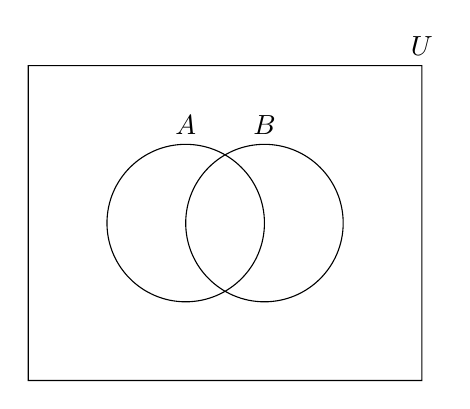
\begin{tikzpicture}[fill=white]
    \draw (0,0) circle (1) (0,1)  node [text=black,above] {$A$}
    (1,0) circle (1) (1,1)  node [text=black,above] {$B$}
    (-2,-2) rectangle (3,2) node [text=black,above] {$U$};
  \end{tikzpicture}
\end{center}

If \(A \subseteq B\) and there is an element of $B$ that is not an element of $A$, meaning \(A \not = B\),
then $A$ is a \textbf{proper subset} of $B$, denoted as \(A \subset B\). An important fact is that
\begin{center}
  \(\mathbb{N} \subset \mathbb{Z} \subset \mathbb{Q} \subset \mathbb{R}\)
\end{center}

\subsection{Sets of sets}
\subsection{Union and Intersection}
\subsection{More set operations}
\subsection{Set identities}
\subsection{Cartesian products}
\subsection{Partitions}
\section{Functions}
\subsection{Definition of functions}
\subsection{Floor and Ceiling functions}
\subsection{Properties of functions}
\subsection{The inverse of a function}
\subsection{Composition of functions}
\subsection{Logarithms and exponents}
\section{Boolean Algebra}
\subsection{An introduction to Boolean Algebra}

\textbf{Boolean Algebra} is a set of rules/operations for working with variables whose values are either 0 or 1.
It corresponds highly to propositional logic.

\textbf{Boolean Multiplication}, denoted by $\cdot$.
\begin{align*}
  \text{Boolean } & \cdot & \text{Logic }           & \land      \\
  0 \cdot 0       & = 0   & \text{F} \land \text{F} & = \text{F} \\
  0 \cdot 1       & = 0   & \text{F} \land \text{T} & = \text{F} \\
  1 \cdot 0       & = 0   & \text{T} \land \text{F} & = \text{F} \\
  1 \cdot 1       & = 1   & \text{T} \land \text{T} & = \text{T}
\end{align*}

\textbf{Boolean Addition}, denoted by $+$.
\begin{align*}
  \text{Boolean } & \cdot & \text{Logic }          & \lor       \\
  0 + 0           & = 0   & \text{F} \lor \text{F} & = \text{F} \\
  0 + 1           & = 1   & \text{F} \lor \text{T} & = \text{T} \\
  1 + 0           & = 1   & \text{T} \lor \text{F} & = \text{T} \\
  1 + 1           & = 1   & \text{T} \lor \text{T} & = \text{T} \\
\end{align*}

\textbf{Boolean Complement}, denoted by $\bar{ }$.
\begin{align*}
  \text{Boolean } & \bar{ } & \text{Logic }  & \lnot      \\
  \bar{0}         & = 1     & \lnot \text{F} & = \text{T} \\
  \bar{1}         & = 0     & \lnot \text{T} & = \text{F} \\
\end{align*}

\begin{center}
  \begin{circuitikz}
    \draw (0,0) to[battery] (0,2)
    to[switch, l=$x$] (2,2)
    to[switch, l=$y$](4,2)
    to[lamp] (4,0) -- (0,0);
    \draw (2,-1) node[] {Shannon Circuit (AND $\cdot$)};
  \end{circuitikz}
  \qquad
  \begin{circuitikz}
    \draw (0,0) to[battery] (0,2) -- (1,2) -- (1,1.5)
    to[switch, l=$x$] (3,1.5) -- (3,2) -- (4,2) to[lamp] (4,0) -- (0,0)
    (1,2) -- (1,2.5)
    to[switch, l=$y$] (3,2.5) -- (3,2);
    \draw (2,-1) node[] {Switching Circuit (OR $+$)};
  \end{circuitikz}
\end{center}

Variables that can have a value of either $1$ or $0$ are called \textbf{Boolean Variables}.
Boolean expressions are made of boolean variables. There are also common shorthand ways of notating operations.
\begin{align*}
  x \cdot y + 1 \cdot \bar{z} & = xy + \bar{z}        \\
  x + z + \overline{0 + y}    & = x + z \cdot \bar{y}
\end{align*}

\begin{center}
  \begin{tabular}{r|c|c}
    \textbf{Law Name} & $+$ OR                                               & $\cdot$ AND                                          \\
    \hline
    Idempotent        & $x + x = x$                                          & $x \cdot x = x$                                      \\
    Associative       & $(x + y) + z = x + (y + z)$                          & $(x \cdot y) \cdot z = x \cdot (y \cdot z)$          \\
    Commutative       & $x + y = y + x$                                      & $x \cdot y = y \cdot x$                              \\
    Distributive      & $x + (y \cdot z) = (x + y) \cdot (x + z)$            & $x \cdot (y + z) = (x \cdot y) + (x \cdot z)$        \\
    Identity          & $x + 0 = x$                                          & $x \cdot 1 = x$                                      \\
    Domination        & $x + 1 = 1$                                          & $x \cdot 0 = 0$                                      \\
    Double Complement & $\overline{\overline{x}} = x$                                                                               \\
    Complement        & $x + \overline{x} =$ 1                               & $x \cdot \overline{x} =$ 0                           \\
    DeMorgan          & $\overline{x + y} = \overline{x} \cdot \overline{y}$ & $\overline{x \cdot y} = \overline{x} + \overline{y}$ \\
    Absorption        & $x + (x \cdot y) = x$                                & $x \cdot (x + y) = x$
  \end{tabular}
\end{center}

\subsection{Boolean functions}
\subsection{Disjunctive and conjunctive normal form}
\subsection{Functional completeness}
\subsection{Boolean satisfiability}
\subsection{Gates and circuits}
\section{Relation and Digraphs}
\subsection{Introduction to binary relations}

A \textbf{Binary Relation} between two sets $A$ and $B$ is a subset $R$ of $A \times B$.
It is binary because it is between two sets.
\[
  \text{for } a \in A \land b \in B, (a,b) \in R \text{ is denoted as } a\text{R}b
\]

For example, consider the relation C between $\mathbb{R}$ and $\mathbb{Z}$:
\[
  x\text{C}y \text{ if } \left\lvert x-y\right\rvert \leq 1, \text{ where } x \in \mathbb{R} \text{ and } y \in \mathbb{Z}
\]
If $A$ and $B$ are finite, then relation R between $A$ and $B$ can be represented by a set of ordered pairs.

\subsubsection{Matrix Representation}
\begin{align*}
  P           & = \{\text{Sue}, \text{Harry}, \text{Sam}\}                       \\
  \text{File} & = \{\text{File A}, \text{File B}, \text{File C}, \text{File D}\}
\end{align*}
\[
  \bordermatrix{ & \text{File A} & \text{File B} & \text{File C} & \text{File D} \cr
    \text{Sue}   & 0 & 1 & 1 & 1 \cr
    \text{Harry} & 1 & 0 & 0 & 0 \cr
    \text{Sam}   & 0 & 0 & 0 & 0 \cr }
\]
\begin{center}
  An element is
  \begin{tabular}{c}
    1 if $p$R$f$ is true \\
    0 if $p$R$f$ is false
  \end{tabular}
\end{center}

\subsubsection{Arrow Diagram}
\begin{align*}
  A & = \{a,b,c,d,e\}                                \\
  R & \subseteq A \times A                           \\
  R & = \{(a,b), (b,c), (e,c), (c,e), (d,a), (d,d)\}
\end{align*}
\begin{center}
  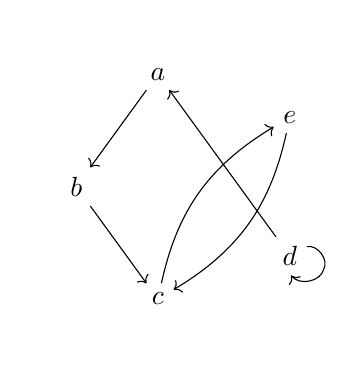
\begin{tikzpicture}
    %VARIABLES
    \pgfmathsetmacro{\gsize}{1.5}
    \pgfmathsetmacro{\gnum}{5}

    \foreach[count=\i] \element in {a,b,c,d,e} { %domain
        \node (\element) at (\i * 360 / \gnum + 180 / \gnum:\gsize) {$\element$};
        \node (\element-) at (\i * 360 / \gnum + 180 / \gnum:\gsize + 0.5) {};
      }
    \foreach \j/\l in {a/b,b/c,d/a} { %a to b
        \draw[->] (\j) -- (\l);
      }
    \foreach \j/\l in {e/c} { %a to b AND b to a
        \draw[->] (\j) to[bend left=20 / \gsize + 10] (\l);
        \draw[->] (\l) to[bend left=20 / \gsize + 10] (\j);
      }
    \foreach \j in {d} { %a to a
        \draw[->] (\j) to[bend left=65] (\j-)
        to[bend left=65] (\j);
      }
  \end{tikzpicture}
\end{center}

\subsubsection{Arrow Diagram vs. Matrix Representation}
\begin{align*}
  A & = \{1,2,3,4\}                                  \\
  R & = \{(1,2), (1,3), (2,2), (2,3), (3,4), (4,3)\}
\end{align*}
\begin{center}
  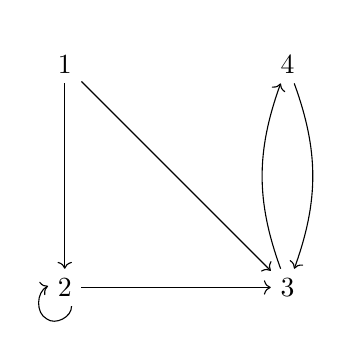
\begin{tikzpicture}
    %VARIABLES
    \pgfmathsetmacro{\gsize}{2}
    \pgfmathsetmacro{\gnum}{4}

    \foreach[count=\i] \element in {1,2,3,4} { %domain
        \node (\element) at (\i * 360 / \gnum + 180 / \gnum:\gsize) {$\element$};
        \node (\element-) at (\i * 360 / \gnum + 180 / \gnum:\gsize + 0.5) {};
      }
    \foreach \j/\l in {1/2,1/3,2/3} { %a to b
        \draw[->] (\j) -- (\l);
      }
    \foreach \j/\l in {3/4} { %a to b AND b to a
        \draw[->] (\j) to[bend left=20 / \gsize + 10] (\l);
        \draw[->] (\l) to[bend left=20 / \gsize + 10] (\j);
      }
    \foreach \j in {2} { %a to a
        \draw[->] (\j) to[bend left=65] (\j-)
        to[bend left=65] (\j);
      }
  \end{tikzpicture}
  \qquad
  $
    \bordermatrix{ & 1 & 2 & 3 & 4 \cr
      1 & 0 & 1 & 1 & 0 \cr
      2 & 0 & 1 & 1 & 0 \cr
      3 & 0 & 0 & 0 & 1 \cr
      4 & 0 & 0 & 1 & 0 \cr }
  $
\end{center}

\subsection{Properties of binary relations}

A binary relation of R on set $A$ is \textbf{Reflective} if for \textit{every} $x \in A$, $x$R$x$.
For Arrow Diagrams, this means the graph contains self-loops:
\begin{center}
  \begin{tikzpicture}
    %VARIABLES
    \pgfmathsetmacro{\gsize}{1}
    \pgfmathsetmacro{\gnum}{2}

    \foreach[count=\i] \element in {a,b} { %domain
        \node (\element) at (\i * 360 / \gnum:\gsize) {$\element$};
        \node (\element-) at (\i * 360 / \gnum:\gsize + 0.5) {};
      }
    \foreach \j in {a,b} { %a to a
        \draw[->] (\j) to[bend left=65] (\j-)
        to[bend left=65] (\j);
      }
  \end{tikzpicture}
\end{center}
For Matrix Representation, this means that the top left to bottom right diagonal are all 1's:
\[
  \bordermatrix{ & a & b & c & d \cr
    a & 1 & - & - & - \cr
    b & - & 1 & - & - \cr
    c & - & - & 1 & - \cr
    d & - & - & - & 1 \cr }
\]

A binary relation of R on set $A$ is \textbf{Anti-reflective} if for \textit{every} $x \in A$, $x$R$x$ is \textit{not} true.
For Arrow Diagrams, this means the graph does not contain self-loops:
\begin{center}
  \begin{tikzpicture}
    %VARIABLES
    \pgfmathsetmacro{\gsize}{1}
    \pgfmathsetmacro{\gnum}{2}

    \foreach[count=\i] \element in {a,b} { %domain
        \node (\element) at (\i * 360 / \gnum:\gsize) {$\element$};
        \node (\element-) at (\i * 360 / \gnum:\gsize + 0.5) {};
      }
  \end{tikzpicture}
\end{center}
For Matrix Representation, this means that the top left to bottom right diagonal are all 0's:
\[
  \bordermatrix{ & a & b & c & d \cr
    a & 0 & - & - & - \cr
    b & - & 0 & - & - \cr
    c & - & - & 0 & - \cr
    d & - & - & - & 0 \cr }
\]

A binary relation of R on set $A$ is \textbf{Symmetric} if and only if for \textit{every} pair $x \in A$, $y \in Y$,
either \textit{both} $x$R$y$ \underline{and} $y$R$x$, or \textit{both} not $x$R$y$ or not $y$R$x$ is true.
For Arrow Diagrams, this means that every arrow has an arrow going the other way:
\begin{center}
  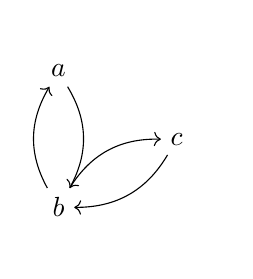
\begin{tikzpicture}
    %VARIABLES
    \pgfmathsetmacro{\gsize}{1}
    \pgfmathsetmacro{\gnum}{3}

    \foreach[count=\i] \element in {a,b,c} { %domain
        \node (\element) at (\i * 360 / \gnum:\gsize) {$\element$};
        \node (\element-) at (\i * 360 / \gnum:\gsize + 0.5) {};
      }
    \foreach \j/\l in {a/b,b/c} { %a to b AND b to a
        \draw[->] (\j) to[bend left=20 / \gsize + 10] (\l);
        \draw[->] (\l) to[bend left=20 / \gsize + 10] (\j);
      }
  \end{tikzpicture}
\end{center}
For Matrix Representation, this means that the top left to bottom right diagonal are all 0's:
\begin{center}
  $
    \bordermatrix{ & a & b & c & d \cr
      a & - & u & v & x \cr
      b & u & - & w & y \cr
      c & v & w & - & z \cr
      d & x & y & z & - \cr }
  $
  where
  \begin{tabular}{c}
    $u \in \{0,1\}$ \\
    $\vdots$        \\
    $z \in \{0,1\}$
  \end{tabular}
\end{center}

A binary relation of R on set $A$ is \textbf{Anti-symmetric} if and only if for \textit{every} pair $x \in A$, $y \in Y$, $x$R$y$ xor $y$R$x$.
For Arrow Diagrams, this means that each arrow does not have an arrow going the other way:
\begin{center}
  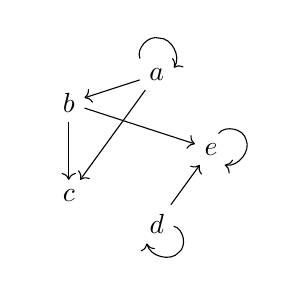
\begin{tikzpicture}
    %VARIABLES
    \pgfmathsetmacro{\gsize}{1}
    \pgfmathsetmacro{\gnum}{5}

    \foreach[count=\i] \element in {a,b,c,d,e} { %domain
        \node (\element) at (\i * 360 / \gnum:\gsize) {$\element$};
        \node (\element-) at (\i * 360 / \gnum:\gsize + 0.5) {};
      }
    \foreach \j/\l in {a/b, b/c, a/c, b/e, d/e} { %a to b
        \draw[->] (\j) -- (\l);
      }
    \foreach \j in {a,e,d} { %a to a
        \draw[->] (\j) to[bend left=65] (\j-)
        to[bend left=65] (\j);
      }
  \end{tikzpicture}
\end{center}
For Matrix Representation, this means that the top left to bottom right diagonal are all 0's:
\begin{center}
  $
    \bordermatrix{ & a & b & c & d \cr
      a & - & \bar{u} & \bar{v} & \bar{x} \cr
      b & u & - & \bar{w} & \bar{y} \cr
      c & v & w & - & \bar{z} \cr
      d & x & y & z & - \cr }
  $
  where
  \begin{tabular}{c}
    $u \in \{0,1\}$ \\
    $\vdots$        \\
    $z \in \{0,1\}$
  \end{tabular}
\end{center}

\subsection{Directed graphs, paths, and cycles}
\subsection{Composition of relations}
\subsection{Graph powers and the transitive closure}
\subsection{Matrix multiplication and graph powers}
\subsection{Partial orders}
\subsection{Strict orders and directed acyclic graphs}
\subsection{Equivalence relations}
\subsection{N-ary relations and relational databases}
\section{Computation}
\subsection{An introduction to algorithms}
An algorithm is a step by step method for solving a problem. It usually includes:
\begin{itemize}
  \item name
  \item brief description
  \item description of input
  \item description of output
  \item sequence of steps to follow
\end{itemize}
Algorithms are often described in \textbf{pseudocode}

\subsubsection*{Assignment operator}
\begin{lstlisting}
  x := y
\end{lstlisting}

\subsubsection*{Return statement}
\begin{lstlisting}
  Return(value)
\end{lstlisting}

\subsubsection*{If-else statement}
\begin{lstlisting}
  If(x = 5), y := 7

  If(condition)             If(condition)
    Step 1                    Step(s)
    Step 2                  Else
    ...                       Step(s)    
    Step n                  End-if
  End-if
\end{lstlisting}

\subsubsection*{For-loop}
\begin{lstlisting}
  For i = s to t    <- first value is s, then s+1, until t is reached
    Step(s)
  End-for
\end{lstlisting}

\subsubsection*{While-loop}
\begin{lstlisting}
  While(condition)
    Step(s)
  End-while
\end{lstlisting}

\subsubsection*{Nested Loops}
\begin{lstlisting}
  Input: sequence a_1, ..., a_n; n

  count := 0
  For i = 1 to n-1
    For j = i+1 to n
      If(a_i = a_j) count := count+1
    End-for
  End-for

  Return(count)
\end{lstlisting}

\subsection{Asymptotic growth of functions}
Consider $f: \mathbb{Z}^+ \rightarrow \mathbb{R}^{\geq}$, where $\mathbb{R}^{\geq}$ denotes the set of non-negative real numbers.
\textbf{Asymptotic growth} of a function $f$ is a measure of how fast the object $f(n)$ grows as the input $n$ grows.
Classification of functions $\mathcal{O}, \Omega,$ and $\Theta$ provide a way to concisely characterize the growth of a function.
\[
  f = \mathcal{O}(g)~~\text{"$f$ is Oh of $g$"}
\]

\subsubsection*{Constant factors}
\begin{align*}
  7n^3 & \rightarrow 7 \text{ is constant factor} \\
  5n^2 & \rightarrow 5 \text{ is constant factor} \\
  3    & \rightarrow 3 \text{ is constant factor}
\end{align*}

\subsubsection*{$\mathcal{O}$ notation}
Let $f$ and $g$ be functions from $\mathbb{Z}^+$ to $\mathbb{R}^{\geq}$.
Then $f=\mathcal{O}(g)$ if there is are positive real numbers $c$ and $n_0$ such that for any $n \in \mathbb{Z}^+$ such that $n \geq n_0$,
\[
  f(n) \leq c \cdot g(n)
\]
Constants $c$ and $n_0$ are said to be a \textit{witness} to the fact $f=\mathcal{O}(g)$

\subsubsection*{$\Omega$ notation}
Let $f$ and $g$ be functions from $\mathbb{Z}^+$ to $\mathbb{R}^{\geq}$.
Then $f=\Omega(g)$ if there is are positive real numbers $c$ and $n_0$ such that for any $n \in \mathbb{Z}^+$ such that $n \geq n_0$,
\[
  f(n) \geq c \cdot g(n)
\]
$f=\Omega(g)$ is read "$f$ is Omega of $g$"

\subsubsection*{Theorem: Relationship of $\mathcal{O}$-notation and $\Omega$-notation}
Let $f$ and $g$ be functions from $\mathbb{Z}^+$ to $\mathbb{R}^{\geq}$. Then $f=\Omega(g) \iff g = \mathcal{O}(f)$

\subsubsection*{$\Theta$ notation}
Let $f$ and $g$ be functions from $\mathbb{Z}^+$ to $\mathbb{R}^{\geq}$.
\[
  f = \Theta(g) \text{ if}: f = \mathcal{O}(g) \land f = \Omega(g)
\]
\begin{itemize}
  \item $f = \Theta(g)$ is read "$f$ is Theta of $g$"
  \item if $f = \Theta(g)$, then $f$ is said to be the \textit{order of} $g$.
\end{itemize}

\subsubsection*{Theorem: Asymptotic Growth of Polynomials}
Let $p(n)$ be a degree-$k$ polynomial of the form
\[
  p(n) = a_{k}n^{k} + a_{k-1}n^{k-1} + \cdots + a_{1}n + a_0 \text{ where } a_k > 0 \\
\]
Then $p(n)$ is $\Theta(n^k)$

\subsubsection*{Asymptotic Growth of Logarithm Functions with Different Bases}
Let $a$ and $b$ be two real numbers greater than 1. Then
\[
  \log_{a}n = \Theta(\log_{b}n)
\]
This is because of the fact that
\[
  \log_{a}n = \log_{a}b \cdot \log_{b}n, \text{ for } a,b > 1
\]
\textit{
  when a function is said to be the $\mathcal{O}$ or $\Omega$ of a logarithm function,
  the base is often omitted because it is understood that as long as the base is greater than 1,
  the value of the base does not matter.
}

\subsubsection*{Growth rate of common functions}
Constant Functions
\begin{itemize}
  \item function that does not depend on $n$ at all
  \item any constant function is $\Theta(1)$
\end{itemize}
Linear
\begin{itemize}
  \item $\Theta(n)$
\end{itemize}
\begin{center}
  \begin{tabular}{l|c}
    Function                                   & Name        \\
    \hline
    $\Theta(1)$                                & Constant    \\
    $\Theta(\log\log n)$                       & Log Log     \\
    $\Theta(\log n)$                           & Logarithmic \\
    $\Theta(n)$                                & Linear      \\
    $\Theta(n \log n)$                         & $n \log n$  \\
    $\Theta(n^2)$                              & Quadratic   \\
    $\Theta(n^3)$                              & Cubic       \\
    $\Theta(n^m)~\text{for}~m\in \mathbb{Z}^+$ & Power       \\
    $\Theta(c^n)~\text{for}~c>1$               & Exponential \\
    $\Theta(n!)$                               & Factorial
  \end{tabular}
\end{center}

\subsubsection*{Rules about Asymptotic Growth}
Let $f$, $g$, and $h$ be functions from $\mathbb{Z}^+$ to $\mathbb{R}^{\geq}$.
\begin{itemize}
  \item if $f=\mathcal{O}(h)$ and $g=\mathcal{O}(h)$, then $f+g=\mathcal{O}(h)$
  \item if $f=\Omega(h)$ and $g=\Omega(h)$, then $f+g=\Omega(h)$
  \item if $f=\mathcal{O}(g)$, $c \cdot f = \mathcal{O}(g)$, $c\in \mathbb{R}^{\geq}$
  \item if $f=\Omega$, $c \cdot f = \Omega(g)$, $c\in \mathbb{R}^{\geq}$
  \item if $f=\mathcal{O}(g)$ and $g=\mathcal{O}(h)$, then $f=\mathcal{O}(h)$
  \item if $f=\Omega(g)$ and $g=\Omega(h)$, then $f=\Omega(h)$
\end{itemize}

\subsection{Analysis of algorithms}
Resources an algorithm requires to run
\begin{itemize}
  \item time, called \textit{time complexity}
  \item space, called \textit{space complexity}
  \item Together called \textbf{computational complexity}
\end{itemize}
\begin{lstlisting}
  ComputeSum
  Input: a_1,a_2,...,a_n  (n is length of sequence)
  Output: the sum of the numbers in the sequence
  sum := 0                  | 1 assignment operation
  For i = 1 to n            | loop iterated n times
    sum := sum + a_i        |   for loop test and increments (2 operations)
  End-for                   |   1 addition and 1 assignment (2 operations)
  Return(sum)               | 1 op for return statement
\end{lstlisting}
\begin{align*}
  f(n) & = 1 + n[2+2] + 1 \\
       & = 1 + 4n + 1     \\
       & = 4n + 2         \\
       & = \mathcal{O}(n)
\end{align*}

\subsubsection*{Growth rates for different input sizes}
\[
  \begin{matrix}
    f(n)       & n=10      & n=50      & n=100                & n=1000                  & \cdots \\
    \log_{2}n  & 3.3 \mu s & 5.6 \mu s & 6.6 \mu s            & 10 \mu s                & \cdots \\
    n          & 10 \mu s  & 50 \mu s  & 100 \mu s            & 1000 \mu s              & \cdots \\
    n\log_{2}n & .03 ms    & .28 ms    & .66 ms               & 10 ms                   & \cdots \\
    n^2        & .1 ms     & 2.5 ms    & 10 ms                & 1 s                     & \cdots \\
    n^3        & 1 ms      & .125 s    & 1 s                  & 16.7 min                & \cdots \\
    2^n        & 1 ms      & 35.7 yrs  & 4 \times 10^{16} yrs & 3.4 \times 10^{287} yrs & \cdots \\
  \end{matrix}
\]

\subsubsection*{Worst-case analysis}
Worst-case analysis evaluates the time complexity on the input which takes the longest time.
\begin{itemize}
  \item upper bound: use $\mathcal{O}$-notation
        \subitem upper bound must apply for every input of size $n$
  \item lower bound: use $\Omega$-notation
        \subitem lower bound need only apply for one possible input of $n$
\end{itemize}
Average-case analysis takes an average running time of algorithm on random inputs.
\begin{lstlisting}
  For(----)
    operations      -> linear (n)
  End-for

  For(----)
    For(----)
      operations    -> quadratic (n^2)
    End-for
  End-for

  For(----)
    For(----)
      For(----)
        operations  -> cubic (n^3)
      End-for
    End-for
  End-for
\end{lstlisting}
and so on. An algorithm runs in \underline{polynomial time} if its time complexity is $\mathcal{O}^k$ for some fixed constant $k$.
An algorithm is considered "efficient" if it runs in polynomial time. For example,
\begin{align*}
  \mathcal{O}(n^5)        & ~\text{is "efficient"}                 \\
  \mathcal{O}(n^{\log n}) & ~\text{is \underline{not} "efficient"}
\end{align*}
\subsection{Finite state machines}
A \textbf{finite state machine} consists of a finite set of states,
with transitions between states triggered by different input actions.
A finite state machine is sometimes called \textit{finite state automation}.
\begin{center}
  \includegraphics[width=.6\linewidth]{resources/coin_push.png}

  states: $Q =$\{locked, unlocked\}
\end{center}
The reaction of a finite state machine to the input received is denoted by a \textbf{transitive function},
often denoted by the symbol '$\delta$'
\[
  \delta([\text{state}],[\text{action}]) = [\text{state}]
\]
In the case of the coin machine,
\[
  \delta(\text{Locked}, \text{Coin}) = \text{Unlocked}
\]
State transition table:
\begin{itemize}
  \item rows represent current state
  \item columns represent possible inputs
  \item each entry for a particular row and column indicate the new state resulting from that state/input combination
\end{itemize}
For example, the state transition table for the coin machine is
\begin{center}
  \begin{tabular}{c|cc}
             & Coin     & Push   \\
    \hline
    Locked   & unlocked & locked \\
    Unlocked & unlocked & locked
  \end{tabular}
\end{center}

\subsubsection*{Components of a Finite State Machine}
\begin{center}
  \begin{tabular}{c|l}
    Notation                           & Description              \\
    \hline
    $Q$                                & finite set of states     \\
    $q_0 \in Q$                        & $q_0$ is the start state \\
    $I$                                & finite set of actions    \\
    $\delta: Q \times I \rightarrow Q$ & transition function
  \end{tabular}
\end{center}

\subsubsection*{FSM with Output}
\begin{align*}
  Q & = \{q_0, q_5, q_{10}, q_{15}, q_{20}\}                           \\
  I & = \{\text{NICKLE}, \text{DIME}, \text{BUY}\}                     \\
  O & = \{\text{Gumball}, \text{Return}, \text{Message}, \text{None}\}
\end{align*}
\begin{center}
  \includegraphics[width=.6\linewidth]{resources/fsm_with_output.png}
\end{center}
An \underline{accepted state} is a state that is okay to end in.
\[
  A \subseteq Q, \text{ Accepted states are a subset of the total states}
\]
Example, recognizing valid password
\begin{center}
  \includegraphics[width=.6\linewidth]{resources/fsm_password.png}

  A valid password must begin with a letter and contain at least one digit.
\end{center}

\subsection{Turing machines}
FSMs are unable to solve even simple computational tasks such as determining whether a binary string has more 0's than 1's.

\subsubsection*{Church-Turing conjecture}
Any problem that can be solved efficiently on any computing device can be solved efficiently by a Turing Machine.

\subsubsection*{Definition of a Turing Machine}
\begin{itemize}
  \item memory is a 1-dimensional tape. \\
        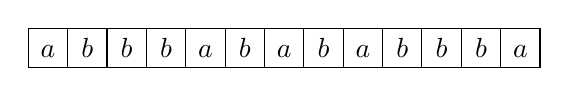
\begin{tikzpicture}
          \pgfmathsetmacro{\x}{0.5};
          \pgfmathsetmacro{\y}{0.5};
          \pgfmathsetmacro{\vset}{0};

          \foreach[count=\i] \element in {a,b,b,b,a,b,a,b,a,b,b,b,a} {
              \draw (\i * \x,0) rectangle ++(\x,\y);
              \node[anchor=south] (\element) at (\i*\x + \x * 0.5, \vset) {$\element$};
            }
        \end{tikzpicture} \\
        example tape for $\{a,b,*\}$
  \item blank symbol (represented by a $*$ symbol)
  \item a \underline{configuration} consists of the contents of the tape, the current state,
        and the tape cell to which the head is currently pointing \\
        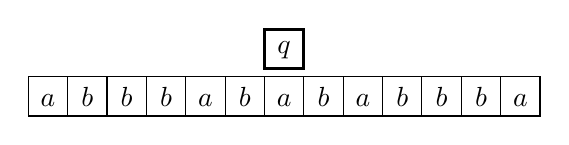
\begin{tikzpicture}
          \pgfmathsetmacro{\x}{0.5};
          \pgfmathsetmacro{\y}{0.5};
          \pgfmathsetmacro{\vset}{0};
          \pgfmathsetmacro{\qset}{7};

          \foreach[count=\i] \element in {a,b,b,b,a,b,a,b,a,b,b,b,a} {
              \draw (\i * \x,0) rectangle ++(\x,\y);
              \node[anchor=south] (\element) at (\i*\x + \x * 0.5, \vset) {$\element$};
            }
          \draw[very thick] (\qset*\x, \y + 0.1) rectangle ++(\x,\y);
          \node[anchor=south] (q) at (\qset*\x + \x*0.5, \y + 0.1) {$q$};
        \end{tikzpicture}
  \item action is determined by a transition function $\delta$
\end{itemize}
Input to Turing Machine is the Input Alphabet, denoted by $\Sigma$,
which much be a subset of the tape alphabet $\Gamma$
\[
  \Sigma \subset \Gamma
\]

\subsubsection*{Components of a Turing Machine}
\begin{center}
  \begin{tabular}{r|l}
    Notation                                                              & Description                                    \\
    \hline
    $Q$                                                                   & finite set of states                           \\
    $\Gamma$                                                              & finite set of tape symbols                     \\
    $\Sigma \subset \Gamma$                                               & A subset of the tape symbols are input symbols \\
    $q_0 \in Q$                                                           & $q_0$ is the start state                       \\
    $q_{acc} \in Q$                                                       & $q_{acc}$ is the accept state                  \\
    $q_{rej} \in Q$                                                       & $q_{rej}$ is the reject state                  \\
    $\delta : Q \times \Gamma \rightarrow Q \times \Gamma \times \{L,R\}$ & Transition Function
  \end{tabular}
\end{center}
Additional Rules
\begin{itemize}
  \item if Turing machine reaches the accept state from a particular input $x$, the Turing machine \textbf{accepts} $x$
  \item if Turing machine reaches the reject state from a particular input $x$, the Turing machine \textbf{rejects} $x$
  \item if Turing machine \textit{accepts} or \textit{rejects} $x$, then the Turing machine \textbf{Halts} on $x$
\end{itemize}
Turing machine that accepts strings with 2 $b$'s
\begin{center}
  \begin{tabular}{c|ccc}
          & $a$         & $b$             & $*$             \\
    \hline
    $q_0$ & $(q_0,a,R)$ & $(q_1,b,R)$     & $(q_{rej},*,L)$ \\
    $q_1$ & $(q_1,a,R)$ & $(q_{acc},b,R)$ & $(q_{rej},*,L)$
  \end{tabular}
\end{center}
\begin{center}
  \begin{tabular}{c}
    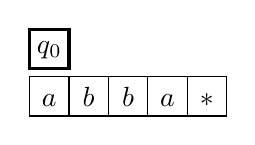
\begin{tikzpicture}
      \pgfmathsetmacro{\x}{0.5};
      \pgfmathsetmacro{\y}{0.5};
      \pgfmathsetmacro{\vset}{0};
      \pgfmathsetmacro{\qset}{1};

      \foreach[count=\i] \element in {a,b,b,a,*} {
          \draw (\i * \x,0) rectangle ++(\x,\y);
          \node[anchor=south] (\element) at (\i*\x + \x * 0.5, \vset) {$\element$};
        }
      \draw[very thick] (\qset*\x, \y + 0.1) rectangle ++(\x,\y);
      \node[anchor=south] (q) at (\qset*\x + \x*0.5, \y + 0.1) {$q_0$};
    \end{tikzpicture} \\
    $\uparrow$ Halts and accepts
  \end{tabular}
  \qquad
  \begin{tabular}{c}
    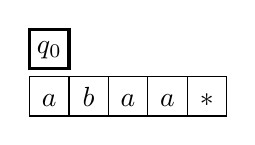
\begin{tikzpicture}
      \pgfmathsetmacro{\x}{0.5};
      \pgfmathsetmacro{\y}{0.5};
      \pgfmathsetmacro{\vset}{0};
      \pgfmathsetmacro{\qset}{1};

      \foreach[count=\i] \element in {a,b,a,a,*} {
          \draw (\i * \x,0) rectangle ++(\x,\y);
          \node[anchor=south] (\element) at (\i*\x + \x * 0.5, \vset) {$\element$};
        }
      \draw[very thick] (\qset*\x, \y + 0.1) rectangle ++(\x,\y);
      \node[anchor=south] (q) at (\qset*\x + \x*0.5, \y + 0.1) {$q_0$};
    \end{tikzpicture} \\
    $\uparrow$ Halts and rejects
  \end{tabular}
\end{center}
Transition function for Turing machine that recognizes powers of 2:
\begin{center}
  \begin{tabular}{c|ccc}
    -           & $a$               & $x$               & $*$               \\
    \hline
    $q_0$       & $(q_{first},*,R)$ & $(q_{rej},*,R)$   & $(q_{rej},x,R)$   \\
    $q_{first}$ & $(q_{even},x,R)$  & $(q_{first},x,R)$ & $(q_{first},*,R)$ \\
    $q_{even}$  & $(q_{odd},a,R)$   & $(q_{even},x,R)$  & $(q_{first},*,R)$ \\
    $q_{odd}$   & $(q_{even},x,R)$  & $(q_{odd},x,R)$   & $(q_{first},*,R)$ \\
    $q_{ret}$   & $(q_{ret},a,R)$   & $(q_{rej},x,R)$   & $(q_{first},*,R)$ \\
  \end{tabular}
\end{center}

\subsection{Decision problems and languages}
\begin{center}
  \begin{tikzpicture}
    %VARIABLES
    \pgfmathsetmacro{\gsize}{1};
    \pgfmathsetmacro{\gnum}{4};

    \foreach[count=\i] \element in {1,2,3,4} { %domain
        \node (\element) at (\i * 360 / \gnum:\gsize) {$\element$};
      }
    \foreach \j/\ls in {1/{2,4},3/{1,4}} {\foreach \l in \ls {\draw[->] (\j) -- (\l);}}
  \end{tikzpicture}
  \begin{tabular}{r|l}
    Symbol set     & ${()~,~;~0~1~2~3~4~5~6~7~8~9}$ \\
    Graph encoding & $4;(1,2)(1,4)(3,1)(3,4)$
  \end{tabular}
\end{center}
Turing Machine can only accept or reject on input.
This limits the class of problems answerable by a turing machine to \textbf{yes} or \textbf{no} problems.
\begin{itemize}
  \item \textbf{Decision Problem}: given a boolean expression, is there
        an assignment to the boolean expression that causes the expression to evaluate to 1?
  \item \textbf{Search Problem}: given a boolean expression, find an assignment to the boolean
        expression that causes the expression to evaluate to 1 if one exists,
        or output that no such assignment exists.
\end{itemize}
If $\Sigma$ is a finite alphabet, then a subset of $\Sigma^*$ is called a \textit{language} over $\Sigma$.

\subsubsection*{Language computed by a Turing Machine}
Let $\Sigma$ denote a finite alphabet and let $L$ be a language over $\Sigma$.
A turing machine $M$ \textbf{computes language L}, or \textbf{decides language L}
if for every $x \in \Sigma$, if $x \in L$, then $M$ rejects $x$ in a finite number of steps.
\begin{itemize}
  \item \textbf{Time Complexity} is measured by how many steps taken by a Turing machine on a particular input.
  \item \textbf{Space Complexity} is measured by the number of tape cells that the turing machine uses in the
        course of it execution on a particular input.
\end{itemize}
A language is \textit{incomputable} if there is no turing machine that computes the language.
\section{Induction and Recursion}
\subsection{Sequences}
A \textbf{sequence} is a special type of function in which the domain
is the set of consecutive integers.

When a function is specified as a sequence, using subscripts to denote input
is more common, so $g_k$ is used instead of $g(k)$

A value $g_k$ is called a \textbf{term}, and $k$ is the \textit{index} of $g_k$

For example:
\begin{align*}
  g_1 & = 3.67 & g_2 & = 2.88 \\
  g_3 & = 3.25 & g_4 & = 3.75
\end{align*}
\[
  g(k) = 3.67, 2.88, 3.25, 3.75
\]

An entire sequence is denoted by $\{gk\}$, whereas $g_k$ is used to denote a
single term in the sequence.

A sequence commonly starts with $0$ or $1$, but it could be \textit{any} integer.
\subsubsection*{Finite sequence}
A sequence with a finite domain is a \textbf{finite sequence}.
In a finite sequence, there is an \textit{initial index $m$} and a \textit{final index $n$}.
\subsubsection*{Infinite sequence}
A sequence with an infinite domain is a \textbf{infinite sequence}.
In an infinite sequence, there is an \textit{initial index m} and the sequence
is defined for indices $k \geq m$:
\[
  a_m, a_{m+1}, a_{m+2}, a_{m+3}, \ldots
\]
A sequence can be specified by an \textbf{explicit formula}, such as $d_k = 2^k$
for $k \geq 1$.
\[
  \{d_k\} = 2,4,8,16, \ldots
\]
\subsubsection*{Increasing and Decreasing Sequences}
\begin{itemize}
  \item a sequence is \textit{increasing} if for every two consecutive indices, $k$
        and $k+1$, $a_k < a_{k+1}$
  \item a sequence is \textit{non-decreasing} if for every two consecutive indices, $k$
        and $k+1$, $a_k \leq a_{k+1}$
\end{itemize}
For example,
\begin{align*}
  2 < 4 < 5 < 6          & ~\text{increasing \textit{and} non-decreasing}     \\
  2 \leq 4 \leq 5 \leq 6 & ~\text{non-decreasing \textit{but} not increasing}
\end{align*}
\textit{The same relationship can be said for \textbf{decreasing} and \textbf{non-increasing}}.
\subsubsection*{Geometric Sequences}
A \textbf{geometric sequence} is a sequence of real numbers where each term is found by taking
the previous term and multiplying it by a fixed number called the \textbf{common ratio}.

For example, with an \textit{initial term}: 4, and \textit{common ratio}: $\frac{1}{2}$,
\[
  4,2,\frac{1}{2},\frac{1}{4}, \ldots
\]
\subsubsection*{Arithmetic Sequence}
An \textbf{arithmetic sequence} is a sequence of real numbers where each term after the initial
term is found by taking the previous term and adding a fixed number called the \textbf{common difference}.

For example, with an \textit{initial value}: 2, and \textit{common difference}: 3,
\[
  2,5,8,11, \ldots
\]

\subsection{Recurrence relations}
A rule that defines a term $a_n$ as a function of previous terms in the sequence is called a
\textbf{recurrence relation}

For example,
\begin{align*}
  a_0 & = a~\text{initial value} \\
  a_n & = d + a_{n-1}
\end{align*}
Fibonacci Sequence:
\begin{align*}
  f_0 & = 0                                     \\
  f_1 & = 1                                     \\
  f_n & = f_{n-1} + f_{n-2}~\text{for}~n \geq 2 \\
\end{align*}
A \textbf{dynamical system} is a system that changes over time. The state of the system
at any point is determined by a set of well-defined rules that depend on the past states
of the system.

\subsection{Summations}


\subsection{Mathematical induction}


\subsection{More inductive proofs}


\subsection{Strong induction and well-ordering}


\subsection{Loop invariants}


\subsection{Recursive definitions}


\subsection{Structural induction}


\subsection{Recursive algorithms}


\subsection{Induction and recursive algorithms}


\subsection{Analyzing the time complexity of recursive algorithms}


\subsection{Divide-and-conquer algorithms: Introduction and mergesort}


\subsection{Divide-and-conquer algorithms: Binary Search}


\subsection{Solving linear homogeneous recurrence relations}


\subsection{Solving linear non-homogeneous recurrence relations}


\subsection{Divide-and-conquer recurrence relations}

\section{Integer Properties}
\subsection{The Division Algorithm}
\subsection{Modular arithmetic}
\subsection{Prime factorizations}
\subsection{Factoring and primality testing}
\subsection{Greatest common factor divisor and Euclid's algorithm}
\subsection{Number representation}
\subsection{Fast exponentiation}
\subsection{Introduction to cryptography}
\subsection{The RSA cryptosystem}
\section{Introduction to Counting}
\subsection{Sum and Product Rules}
\subsection{The Bijection Rules}
\subsection{The generalized product rule}
\subsection{Counting permutations}
\subsection{Counting subsets}
\subsection{Subset and permutation examples}
\subsection{Counting by complement}
\subsection{Permutations with repetitions}
\subsection{Counting multisets}
\subsection{Assignment problems: Balls in bins}
\subsection{Inclusion-exclusion principle}
\section{Advanced Counting}
\subsection{Generating permutations}
There are situations in which it is necessary to generate, not just count, all permutations of a set or subsets of a given size.

\subsubsection*{Lexicographic Order}
A well-defined order imposed on the n-tuples is useful to systematically generate all the elements in a set of n-tuples. Generating the n-tuples in the set from smallest to largest ensures that each n-tuple is generated exactly once.

\bld{Lexicographic order} is a way or ordering n-tuples in which two n-tuples are compared according to the first entry where they differ. An example of such ordering is the word in a dictionary.

\subsubsection*{Generating Permutations}
A \bld{permutation} of the set $\{1,2,\ldots,n\}$ is an ordered n-tuple in which each number in $\{1,2,\ldots,n\}$ appears exactly once. For example, $(2,5,1,4,3)$ is a permutation of the set $\{1,2,3,4,5\}$.

\subsubsection*{Generating r-subsets of a set}
Unlike sequences or n-tuples, the order in which the elements of a set or subset are written does not matter. Sets can be ordered lexicographically by first sorting the elements in increasing order and then comparing the two sets as if they were ordered sequences. For example, $\{2,3,11\} < \{2,5,6\}$, because the first element is the same in both sets but in the second element $3 < 5$.

\subsection{Binomial coefficients and combinatorial identities}
An \bld{identity} is a theorem stating that two mathematical expressions are equal.

\subsubsection*{Theorem: A Simple Combinatorial Identity}
For any non-negative integers $n \tand k \tsuchthat k \leq n$:
\[
  \binom{n}{k} = \binom{n}{n-k}
\]

A proof that makes use of counting principles is called a \bld{combinatorial proof}. Combinatorial proofs usually involve defining a set $S$ and counting the number of elements in $S$ to get a mathematical expression for the number of items in the set. Every combinatorial proof of an identity uses a bijection implicitly as part of the argument.

\subsubsection*{Theorem: The Binomial Theorem}
For any non-negative integer $n$ and any real numbers $a \tand b$:
\[
  (a + b)^n = \sum_{k=0}^{n} \binom{n}{k} a^{n-k}b^k = \sum_{k=0}^{n} \binom{n}{k} a^kb^{n-k}
\]
The coefficients $\binom{n}{k}$ are called binomial coefficients.

For the case $n = 5$, the Binomial Theorem says that
\begin{align*}
  (a+b)^5 & = \binom{5}{0}a^5 + \binom{5}{1}a^4b + \binom{5}{2}a^3b^2 + \binom{5}{3}a^2b^3 + \binom{5}{4}ab^4 + \binom{5}{5}b^5 \\
          & = a^5 + 5a^4b + 10a^3b^2 + 10a^2b^3 + 5ab^4 + b^5
\end{align*}

The Binomial Theorem can also be used to obtain combinatorial identities. For example, by plugging in $a=b=1$, the Binomial Theorem yields the identity below.
\[
  2^n = \sum_{k=0}^{n} \binom{n}{k}
\]

Similarly, by letting $a=-1 \tand b=1$, and requiring that $n$ be positive, the left hand side of the Binomial Theorem becomes 0. The right hand side of the Binomial Theorem becomes:
\[
  0 = \sum_{k=0}^{n}(-1)^k \binom{n}{k}
\]
In the expanded form,
\[
  \binom{n}{0} - \binom{n}{1} + \binom{n}{2} - \binom{n}{3} + \cdots + (-1)^n \binom{n}{n} = 0
\]

\subsubsection*{Pascal's Triangle}
The $17^{th}$ century French mathematician, Blaise Pascal, developed a triangular chart that contains all the number of the form $\binom{n}{k}$. The chart, now known as Pascal's Triangle, can be used to derive the value of a particular $\binom{n}{k}$. The $n^{th}$ row of Pascal's Triangle contains the $n+1$ binomial coefficients of the form $\binom{n}{k}$ as shown in the figure below.
\[
  \begin{array}{cccccccccc}
    n=0 &              &              &              &              & \binom{0}{0} &              &              &                             \\
    n=1 &              &              &              & \binom{1}{0} &              & \binom{1}{1} &              &                             \\
    n=2 &              &              & \binom{2}{0} &              & \binom{2}{1} &              & \binom{2}{2} &                             \\
    n=3 &              & \binom{3}{0} &              & \binom{3}{1} &              & \binom{3}{2} &              & \binom{3}{3}                \\
    n=4 & \binom{4}{0} &              & \binom{4}{1} &              & \binom{4}{2} &              & \binom{4}{3} &              & \binom{4}{4} \\
  \end{array}
\]

\subsubsection*{Theorem: Pascal's Identity}
For any positive $n \tand k \tsuchthat k < n$:
\[
  \binom{n}{k} = \binom{n-1}{k-1} + \binom{n-1}{k}
\]

\subsection{The pigeonhole principle}
The pigeonhole principle is a mathematical tool used to establish that repetitions are guaranteed to occur in certain sets and sequences. The \bld{pigeonhole principle} says that if $n+1$ pigeons are placed in $n$ boxes, then there must be at least one box with more than one pigeon. The diagram below shows 10 pigeons, represented as $P$, in 9 boxes.
\begin{center}
  \begin{tabular}{ccc}
    $P$ & $P$ & $P$   \\
    $P$ & $P$ & $P,P$ \\
    $P$ & $P$ & $P$
  \end{tabular}
\end{center}

\subsubsection*{Theorem: The Pigeonhole Principle}
If a function $f$ has a domain of size at least $n+1$ and a target of size at most $n$, where $n$ is a positive integer, then there are two elements in the domain that map to the same element in the target (i.e., the function is not one-to-one)

\subsubsection*{Theorem: The Generalized Pigeonhole Principle}
Consider a function whose domain has at least $n$ elements and whose target has $k$ elements, for $n \tand k$ positive integers. Then there is an element $y$ in the target such that $f$ maps at least $\lceil n/k \rceil$ elements in the domain to $y$.

\subsubsection*{Theorem: Converse of the Generalized Pigeonhole Principle}
Suppose that a function $f$ maps a set of $n$ elements to a target with $k$ elements, where $n \tand k$ are positive integers. In order to guarantee that there is an element $y$ in the target to which $f$ maps to at least $b$ elements from the domain, then $n$ must be at least $k(b-1)+1$.

\subsection{Generating functions}
Generating functions are a powerful tool that can be used to solve a variety of problems related to counting and recurrence relations. A \bld{generating function} is a way of representing a sequence of number as a n algebraic function in which each term in the sequence is a coefficient of an $x^j$ term in the function. The advantage of representing sequences algebraically is that there are many techniques from algebra that can be used to manipulate functions which then leads to insight about the sequences they represent.

The sequence $f_0,f_1,f_2,f_3,\ldots$ is represented by the generating function
\[
  F(x) = f_0 + f_1x + f_2x^2 + f_3x^3 + \cdots
\]

The numbers in the sequence are the coefficients of the terms in $F(x)$. For the sequence $1,1,1,1,\ldots$ is represented by the generating function
\[
  H(x) = 1 + x + x^2 + x^3 + \cdots
\]
When $|x|<1$ for $H(x)$ the sum is finite and has a closed form of
\[
  H(x) = \sum_{j=0}^{\infty} x^j = \frac{1}{1-x}
\]
Additionally, for the partial sum up to $x^k$,
\[
  \sum_{j=0}^{k} x^j = \frac{1-x^k}{1-x}
\]

\subsubsection*{Using Generating Functions for Counting}
One of the primary uses for generating functions is to help solve counting problems. In general, $f_j$ is the number of way to select a subset of $j$ objects.

Consider the situation in which there is a set of two apples and one banana. The apples are indistinguishable, so selecting one apple is the same as selecting the other.
\begin{center}
  \includegraphics[width=.6\linewidth]{resources/11_two_apple_one_banana.png}
\end{center}

If the set from which the subsets are selected is an infinite set, then the resulting sequence is also infinite.

\subsubsection*{Summary of Generating Functions}
\begin{center}
  \begin{tabular}{|c|c|c|}
    \hline
    Description                                                  & Long Form                            & Short Form                               \\
    \hline
    Infinite supply of one kind of item                          & $1 + x + x^2 + x^3 + \cdots$         & ${\displaystyle \frac{1}{1-x}}$          \\
    \hline
    Selecting from a set of $n$ identical items                  & $1 + x + x^2 + x^3 + \cdots + x^n$   & ${\displaystyle \frac{1-x^{n-1}}{1-x}}$. \\
    \hline
    Infinite supple of identical items grouped in batches of $k$ & $1 + x^k + x^{2k} + x^{3k} + \cdots$ & ${\displaystyle \frac{1}{1-x^k}}$        \\
    \hline
    Infinite supple of 2 different kinds of items                & $1 + 2x + 3x^2 + 4x^3 + \cdots$      & ${\displaystyle \frac{1}{(1-x)^2}}$      \\
    \hline
  \end{tabular}
\end{center}

\subsubsection*{Products of Generating Functions}
Generating functions become very useful when different sets of objects are combined together into larger sets.

For example, if we are selecting subsets of apples from a set of 3 apples, the generating function is $A(x) = 1 + x + x^2 + x^3$, and if we are selecting bananas from a set of 2 bananas, the generating function is $B(x) = 1 + x + x^2$. Now suppose we pool the three apples and two bananas into a set of five pieces of fruit and ask 'how many ways can one select a set of fruit from the collection of five pieces of fruit?'

The power of generating functions is illustrated in the fact that if we take the product of $A(x)$, the generating function for apples, and $B(x)$, the generating function for bananas, to get $A(x)B(x)$, then the resulting product is the generating function for the pooled set of five pieces.
\[
  A(x)B(x) = (1 + x + x^2 + x^3)(1 + x + x^2) = 1 + 2x + 3x^2 + 3x^3 + 2x^4 + x^5
\]
Note that the rule of multiplying generating function only works when the two sets of objects being combined are \itl{distinct}. The rule would not work for combining two sets of indistinguishable apples.

Now suppose that we add oranges to the set of selections. There are three oranges, but they come wrapped in a single pack, so one can select zero or three oranges, but not one or two. The generating function for oranges is $O(x) = 1 + x^3$. Again, we can take the product of the generating functions to solve, 'how many ways are there to select subsets of fruit of a particular size?'
\[
  A(x)B(x)O(x) = 1 + 2x + 3x^2 + 4x^3 + 4x^4 + 4x^5 + 3x^6 + 2x^7 + x^8
\]
The coefficient of $x^5$ in the generating function for the whole set of fruit is 4, so there are 4 ways to select 5 pieces of fruit.
\section{Discrete Probability}
\subsection{Probability of an event}
\subsection{Unions and complements of events}
\subsection{Conditional probability and independence}
\subsection{Bayes' Theorem}
\subsection{Random variables}
\subsection{Expectation of random variables}
\subsection{Linearity of expectations}
\subsection{Bernoulli trials and the binomial distribution}
\section{Graphs}
\subsection{Introduction to Graphs}
Graphs are fundamental objects in discrete mathematics that model relationships between pairs of objects. Graphs arise in a wide array of disciplines but play an especially important role in computer science.

In an \bld{undirected graph}, the edges are unordered pairs of vertices, which is useful for modeling relationships that are symmetric. A graph consists of a pair of sets $(V,E)$, where $V$ is a set of vertices and $E$ is a set of edges. A graph is \bld{finite} if the vertex set is finite. A single element of $V$ is called a \bld{vertex} and is usually represented pictorially by label, or a dot with a label. Each edge in $E$ is a set of two vertices from $V$ and is drawn as a line connecting the two vertices.
\begin{center}
  \begin{tikzpicture}
    %VARIABLES
    \pgfmathsetmacro{\gsize}{1};
    \pgfmathsetmacro{\gnum}{5};

    \foreach[count=\i] \element in {a,b,c,d,e} { %domain
        \node (\element) at (\i * 360 / \gnum:\gsize) {$\element$};
        \node (\element-) at (\i * 360 / \gnum:\gsize + 0.5) {};
      }
    \foreach \j/\l in {a/b,a/c,b/c,b/e,c/d,d/e} { %a to b
        \draw (\j) -- (\l);
      }
    \node[anchor=east] (name) at (145:\gsize+.5) {An undirected graph}; %relation name
  \end{tikzpicture}
\end{center}
In the above graph, two edges cross each other, but there is no vertex at the crossing. The crossing is just a byproduct of how the graph is drawn on a two-dimensional surface. The graph above can be described by listing the vertex set and the edge set:
\begin{align*}
  V & = \{a,b,c,d,e\}                                       \\
  E & = \{\{a,b\},\{a,c\},\{b,c\},\{b,e\},\{c,d\},\{d,e\}\}
\end{align*}
A graph may appear to be disconnected into more than one piece but is still considered to be one graph. Here are two graphs, each with 5 vertices.
\begin{center}
  \begin{tikzpicture}
    %VARIABLES
    \pgfmathsetmacro{\gsize}{1};
    \pgfmathsetmacro{\gnum}{5};

    \foreach[count=\i] \element in {a,b,c,d,e} { %domain
        \node (\element) at (\i * 360 / \gnum:\gsize) {$\element$};
        \node (\element-) at (\i * 360 / \gnum:\gsize + 0.5) {};
      }
    \foreach \j/\l in {a/b,c/d,d/e} { %a to b
        \draw (\j) -- (\l);
      }
    \node[anchor=east] (name) at (145:\gsize+.5) {Graph $A$}; %relation name
  \end{tikzpicture}
  \begin{tikzpicture}
    %VARIABLES
    \pgfmathsetmacro{\gsize}{1};
    \pgfmathsetmacro{\gnum}{5};

    \foreach[count=\i] \element in {a,b,c,d,e} { %domain
        \node (\element) at (\i * 360 / \gnum:\gsize) {$\element$};
        \node (\element-) at (\i * 360 / \gnum:\gsize + 0.5) {};
      }
    \node[anchor=east] (name) at (145:\gsize+.5) {Graph $B$}; %relation name
  \end{tikzpicture}
\end{center}
\bld{Parallel edges} are multiple edges between the same pair of vertices. In defining graphs with parallel edges, it \itl{might} be important to have additional label besides the two endpoints to specify an edge in order to distinguish between different parallel edges. A graph can also have a \bld{self-loop} which is an edge between a vertex, and itself.
\begin{center}
  \begin{tikzpicture}
    %VARIABLES
    \pgfmathsetmacro{\gsize}{1};
    \pgfmathsetmacro{\gnum}{4};

    \foreach[count=\i] \element in {a,b,c,d} { %domain
        \node (\element) at (\i * 360 / \gnum:\gsize) {$\element$};
        \node (\element-) at (\i * 360 / \gnum:\gsize + 0.5) {};
      }
    \foreach \j/\l in {a/c,b/d,c/d} { %a to b
        \draw (\j) -- (\l);
      }
    \foreach \j/\l in {a/b} { %a to b TWICE (parallel edges)
        \draw (\j) to[bend left=20 / \gsize + 10] (\l);
        \draw (\l) to[bend left=20 / \gsize + 10] (\j);
      }
    \foreach \j in {c} { %a to a
        \draw (\j) to[bend left=65] (\j-)
        to[bend left=65] (\j);
      }
    \node[anchor=east] (name) at (145:\gsize+.5) {A graph with parallel edges and a self-loop}; %relation name
  \end{tikzpicture}
\end{center}
If a graph does not have parallel edges or self-loops, it is said to be a \bld{simple graph}.

\subsubsection*{Graph terminology}
\begin{center}
  \begin{tikzpicture}
    %VARIABLES
    \pgfmathsetmacro{\gsize}{1};
    \pgfmathsetmacro{\gnum}{5};

    \foreach[count=\i] \element in {a,b,c,d,e} { %domain
        \node (\element) at (\i * 360 / \gnum:\gsize) {$\element$};
        \node (\element-) at (\i * 360 / \gnum:\gsize + 0.5) {};
      }
    \foreach \j/\l in {a/b,a/c,b/c,b/e,c/d,d/e} { %a to b
        \draw (\j) -- (\l);
      }
    \node[anchor=east] (name) at (145:\gsize+.5) {Undirected graph example}; %relation name
  \end{tikzpicture}
\end{center}
\begin{itemize}
  \item If there is an edge between two vertices, they are said to be \bld{adjacent}. In the graph above, $d \tand e$ are adjacent, but $d \tand b$ are not adjacent.
  \item Vertices $b \tand e$ are the \bld{endpoints} of edge $\{b,e\}$. The edge $\{b,e\}$ is \bld{incident} to vertices $b tand e$.
  \item A vertex $c$ is a \bld{neighbor} of vertex $b$ if and only if $\{b,c\}$ is an edge. In the graph above, the neighbors of $b$ are the vertices $a,c, \tand e$.
  \item In a simple graph, the \bld{degree} of a vertex is the number of neighbors it has. In the graph above, the degree of $b$ is 3 and the degree of vertex $a$ is 2. The degree of vertex $b$ is denoted by $\deg(b)$.
  \item The \bld{total degree} of a graph is the sum of the degrees of all of the vertices. The total degree of the above graph is $2 + 3 + 3 + 2 + 2 = 12$.
  \item In a \bld{regular graph}, all the vertices have the same degree. In a \bld{$d$-regular graph}, all the vertices have degree $d$. The graph above is not regular because $\deg(a) \neq \deg(b)$. However, the graph below is 3-regular.
\end{itemize}
\begin{center}
  \includegraphics[width=.2\linewidth]{resources/3-regular graph.png}
\end{center}
\begin{itemize}
  \item A graph $H = (V_H,E_H)$ is a \bld{subgraph} of a graph $G = (V_G,E_G)$ if $V_H \subseteq V_G \tand E_H \subseteq E_G$. Note that any graph $G$ is a subgraph of itself.
\end{itemize}
\begin{center}
  \includegraphics[width=.6\linewidth]{resources/H is a subgraph of G.png}
\end{center}

\subsubsection*{Theorem: Number of Edges and Total Degree}
Let $G = (V,E)$ be an undirected graph, simple or not. Then, twice the number of edges is equal to the total degree:
\[
  \sum_{v \in V} \deg(v) = 2 \cdot |E|
\]

\subsubsection*{Common Graphs}
Some graphs with special structure are given their own name and notation because they come up so frequently in graph theory.
\begin{center}
  \includegraphics[width=0.6\linewidth]{resources/common graphs.png}
\end{center}
For the definition of all of these graphs, $n \in \bb{Z}^+$.
\begin{itemize}
  \item $K_n$ is called the \bld{complete graph} on $n$ vertices. $K_n$ has an edge between every pair of vertices. $K_n$ is sometimes called a \bld{clique} of size $n$ or an \bld{$n$-clique}.
  \item $C_n$ is called a cycle on $n$ vertices. The edges connect the vertices in a ring. Note that $C_n$ is well defined only for $n \geq 3$.
  \item The $n$-dimensional hypercube, denoted $Q_n$, has $2^n$ vertices. Each vertex is label with an $n$-bit string. Two vertices are connected by an edge if their corresponding labels differ only by one bit.
  \item $K_{n,m}$ has $n+m$ vertices, and $2nm$ edges. The vertices are divided into two sets: one with $m$ vertices and one set with $n$ vertices. There are no edges between vertices in the same set, but there is an edge between every vertex in one set and every vertex in the other set.
\end{itemize}

\subsection{Graph representations}
\begin{center}
  \includegraphics[width=0.5\linewidth]{resources/two similar graphs.png}
\end{center}
These two graphs look different, but that is only because they are drawn differently. The two graphs are actually the same graph because they have the same vertex and edge sets as shown below:
\begin{align*}
  V & = \{a,b,c,d,e\}                                       \\
  E & = \{\{a,b\},\{a,c\},\{b,c\},\{b,e\},\{c,d\},\{d,e\}\}
\end{align*}
The way a graph is drawn is not part of the graph itself.

\subsubsection*{Adjacency List Representation for Graphs}
In the \bld{adjacency list representation} of a graph, each vertex has a list of all its neighbors. Note that since the graph is undirected if vertex $a$ is in $b$'s list of neighbors, then $b$ must also be in $a$'s list of neighbors.

If a graph is represented using adjacency lists, the time required to list the neighbors of a vertex $v$ is proportional to $\deg(v)$, the number of vertices to be listed. In order to determine if $\{a,b\}$ is an edge, it is necessary to scan the list of $a$'s neighbors or the list of $b$'s neighbors. In the worst case, the time required is proportional to the larger of $\deg(a)$ or $\deg(b)$.

\subsubsection*{Matrix Representation for Graphs}
The \bld{matrix representation} for a graph with $n$ vertices is an $n \times n$ matrix whose entries are all either $0 \tor 1$, indicating whether or not each edge is present. The matrix representation of an undirected graph is symmetric.
\begin{center}
  \begin{tikzpicture}
    %VARIABLES
    \pgfmathsetmacro{\gsize}{1};
    \pgfmathsetmacro{\gnum}{5};

    \foreach[count=\i] \element in {a,b,c,d,e} { %domain
        \node (\element) at (\i * 360 / \gnum:\gsize) {$\element$};
        \node (\element-) at (\i * 360 / \gnum:\gsize + 0.5) {};
      }
    \foreach \j/\l in {a/b,a/c,b/c,b/e,c/d,d/e} { %a to b
        \draw (\j) -- (\l);
      }
    \node[anchor=east] (name) at (145:\gsize+.5) {}; %relation name
  \end{tikzpicture} $~~\Rightarrow~~$
  $
    \begin{bmatrix}
      0 & 1 & 1 & 0 & 0 \\
      1 & 0 & 1 & 0 & 1 \\
      1 & 1 & 0 & 1 & 0 \\
      0 & 0 & 1 & 0 & 1 \\
      0 & 1 & 0 & 1 & 0
    \end{bmatrix}
  $
\end{center}

\subsection{Graph isomorphism}
Two graphs are said to be \bld{isomorphic} if there is a correspondence between the vertex sets of each graph such that there is an edge between two vertices of one graph if and only if there is an edge between the corresponding vertices of the second graph. Essentially, the graphs are not identical but the vertices can be relabeled so that they are identical.

\subsubsection*{Definition of Isomorphic Graphs}
Let $G = (V,E) \tand G'=(V',E')$. $G \tand G'$ are isomorphic if there is a bijection $f: V \rightarrow V'$ such that for every pair of vertices $x,y \in V$, $\{x,y\} \in E$ if and only if $\{f(x), f(y)\} \in E'$. The function $f$ is called an \bld{isomorphism} from $G \tto G'$.

\begin{center}
  \includegraphics[width=0.4\linewidth]{resources/isomorphic graphs 1.png}
\end{center}
The following function is an isomorphism from the vertices of $G_1 \tto G_2$:
\[
  f(1) = d \qquad f(2) = a \qquad f(3) = c \qquad f(4) = b
\]

\subsubsection*{Theorem: Vertex Degree Preserved under Isomorphism}
Consider two graphs, $G \tand G'$. Let $f$ be an isomorphism from $G \tto G'$. For each vertex $v \tin G$, the degree of vertex $v \tin G$ is equal to the degree of vertex $f(v) \tin G'$.

\subsubsection*{}
The \bld{degree sequence} of a graph is a list of the degree of all of the vertices in non-increasing order.
\begin{center}
  \includegraphics[width=0.7\linewidth]{resources/degree-sequence.png}
\end{center}

\subsubsection*{Theorem: Degree Sequence Preserved under Isomorphism}
The degree sequence of a graph is preserved under isomorphism.


\subsection{Walks, trails, circuits, paths, and cycles}
A \bld{walk} from $v_0 \tto v_l$ in an undirected graph $G$ is a sequence of alternating vertices and edges that starts and ends with a vertex:
\[
  \langle v_0,\{v_0,v_1\},v_1,\{v_1,v_2\},\ldots,v_{\ell-1},\{v_{\ell-1},v_\ell\},v_\ell\rangle
\]
Since the edges in a walk are completely determined by the vertices, a walk can also be denoted by the sequence of vertices:
\[
  \langle v_0,v_1,\ldots,v_\ell \rangle.
\]
However, keep in mind the sequence of vertices is a walk only if $\{v_{j-1},v_j\} \in E$ for each $j = 1,2,\ldots,\ell$. The \bld{length of a walk} is $\ell$, the number of edges in the walk. An \bld{open walk} is a walk in which the first and last vertices are not the same. A \bld{closed walk} is a walk in which the first and last vertices are the same.
\begin{itemize}
  \item A \bld{trail} is a walk in which no \itl{edge} occurs more than once.
  \item A \bld{path} is a walk in which no \itl{vertex} occurs more than once.
  \item A \bld{circuit} is a closed \itl{trail}.
  \item A \bld{cycle} is a \itl{circuit} is length at least 1 in which no vertex occurs more than once, except the first and last vertices which are the same.
\end{itemize}
Here are some examples of closed walks:
\begin{itemize}
  \item $\langle A,C,D,A \rangle$ is a \itl{trail}, a \itl{circuit}, and a \itl{cycle}.
  \item $\langle A,C,B,A,D,E,A \rangle$ is a \itl{trail} and a \itl{circuit}.
  \item $\langle A,B,A \rangle$ is \bld{not} a trail, circuit, or a cycle.
\end{itemize}
Since paths and cycles do not have any repeated edges, if a graph is simple, any cycle \itl{must} have length at least 3. The sequence $\langle v \rangle$ is not a cycle because a cycle, by definition, must have length at least 1. The sequence $\langle v,v \rangle$ is only a walk if there is a self-loop at vertex $v$.

\subsection{Graph connectivity}
Two vertices, $v \tand w$, are \bld{connected} if there is a path from $v \tto w$ (and thus also a path from $w \tto v$). A vertex is always considered to be connected to itself. The property of being connected can be extended to sets of vertices and the entire graph:
\begin{itemize}
  \item A set of vertices in a graph is said to be connected if every pair of vertices in the set is connected.
  \item A graph is said to be connected if every pair of vertices in the graph is connected, and is \bld{disconnected} otherwise.
\end{itemize}
A \bld{connected component} consists of a \itl{maximal} set of vertices that are connected as well as all the edges between two vertices in the set. A vertex that is not connected with any other vertex is called an \bld{isolated vertex} and is therefore a connected component with only one vertex.
\begin{center}
  \includegraphics[width=0.6\linewidth]{resources/connected components example.png}
\end{center}

\subsubsection*{k-Connectivity}
In some networks, it is important to be able to guarantee connectivity, even if one or more vertices or edges are removed from a graph. The definition of connectivity can be extended to encompass resilience to vertex or edge failures.

\subsubsection*{Definition of a K-vertex-connected Graph}
An undirected graph $G$ is \bld{$k$-vertex-connected} if the graph contains at least $k + 1$ vertices and remains connected after any $k - 1$ vertices are removed from the graph. The \bld{vertex connectivity} of a graph is the largest $k$ such that the graph is $k$-vertex-connected. The vertex connectivity of a graph $G$ is denoted $\kappa(G)$.

The vertex connectivity of a graph is the minimum number of vertices whose removal disconnects the graph into more than one connected component.

When the graph is a complete graph, there is no set of vertices whose removal disconnects the graph. For the special case of $K_n$, the vertex connectivity $\kappa(K_n)$ is just defined to be $n - 1$.

\subsubsection*{Definition of a K-edge-connected Graph}
An undirected graph G is \bld{$k$-edge-connected} if removing any $k - 1$ or fewer edges results in a connected graph. The \bld{edge connectivity} of a graph is the largest $k$ such that the graph is $k$-edge-connected. The edge connectivity of a graph G is denoted $\lambda(G)$.

The edge connectivity of a graph is the minimum number of edges whose removal disconnects the graph into more than one connected component.

\subsubsection*{Theorem: Upper bound for Vertex and Edge Connectivity}
Let $G$ be an undirected graph. Denote the minimum degree of any vertex in $G$ by $\delta(G)$. Then,
\begin{align*}
  \kappa(G)  & \leq \delta(G)~~~\tand \\
  \lambda(G) & \leq \delta(G).
\end{align*}

\subsection{Euler circuits and trails}
An \bld{Euler circuit} is a circuit that contains every edge and every vertex. Note that a circuit, by definition, has no repeated edges, so an Euler circuit contains each edge exactly once.
\begin{center}
  \includegraphics[width=0.2\linewidth]{resources/euler circuit example.png}
  Euler circuit: $\langle a,b,c,d,e,b,d,a \rangle$
\end{center}

\subsubsection*{Theorem: Characterization of Graphs that have an Euler Circuit}
An undirected graph $G$ has an Euler circuit if and only if $G$ is connected and every vertex in $G$ has even degree.
\[
  G~\text{has an Euler circuit}~\leftrightarrow G~\text{is connected and every vertex in $G$ has even degree}.
\]

\subsubsection*{Procedure to find a circuit in a Graph}
\begin{lstlisting}
Find a vertex w, that is not an isolated vertex.
Select any edge {w,x} incident to w.
(Since w is not isolated, there is always at least one such edge.)
Current trail T := <w,x>
last := x
While there is an edge {last, y} that has not been used in T:
  Add y to the end of T
  last := y
\end{lstlisting}

\subsubsection*{Procedure to find an Euler circuit in a Graph}
Use the procedure above to find any circuit in $G$. Call the circuit $C$. The algorithm continues to iterate the following steps until all the edges in $G$ are included in $C$:
\begin{enumerate}
  \item Remove all edges in $C$ from $G$. Remove any isolated vertices from $G$. Call the resulting graph $G'$.
  \item Find a vertex $w$ that is in $G' \tand C$.
  \item Find a circuit in $G'$ that begins and ends with $w$. Call the circuit $C'$.
  \item Combine circuit $C \tand C'$. Suppose $C$ starts and ends at vertex $v$. Create a new circuit that starts at $v$ and follows the edges in $C$ until $w$ is reached. The new circuit then follows the edges in $C'$ back to $w$ and then follows the rest of the edges in $C$ back to $v$. The new circuit is renamed $C$ for the next iteration.
\end{enumerate}


\subsubsection*{Euler trail}
An \bld{Euler trail} is an open trail that includes each edge. Note that a trail, by definition, has no repeated edges, so an Euler trail contains each edge exactly once. In an open trail, the first and last vertices are not equal.

\subsubsection*{Theorem: Characterizations of graphs that have an Euler trail}
An undirected graph $G$ has an Euler trail if and only if $G$ is connected and has exactly two vertices with odd degree. The Euler trail begins and ends with the vertices of odd degree.
\[
  G~\text{has an Euler trail}~\leftrightarrow G~\text{is connected and has exactly two vertices with odd degree}.
\]

\subsection{Hamiltonian cycles and paths}
A \bld{Hamiltonian cycle} in an undirected graph is a cycle that includes every vertex in the graph. Note that a cycle, by definition, has no repeated vertices or edges, except for the vertex which is at the beginning and end of the cycle. Therefore, every vertex in the graph appears exactly once in a Hamiltonian cycle, except for the vertex which is at the beginning and end of the cycle. A \bld{Hamiltonian path} in an undirected graph is a path that includes every vertex in the graph. Note that a path, by definition, has no repeated vertices or edges, so every vertex appears exactly once in a Hamiltonian path.

Note that a Hamiltonian cycle can be transformed into a Hamiltonian path by deleting the last vertex. Therefore if a graph has a Hamiltonian cycle, then the graph also has a Hamiltonian path.

Unlike Euler circuits and trails, there are no known conditions describing exactly which graphs have a Hamiltonian cycle or path. However, there are some cases in which a graph that does have a Hamiltonian cycle or path has a certain property.
\begin{itemize}
  \item Any graph that has a vertex with degree 1 does not have a Hamiltonian cycle.
  \item For $n \geq 3$, $K_n$ has a Hamiltonian cycle.
\end{itemize}

\subsection{Planar graphs}
Placing graphs on two-dimensional surfaces to avoid crossings is a classic problem in graph theory. The problem also arises in the field of graph drawing in which the goal is to draw complex graphs in a way that helps people visualize structure and patterns.

An \bld{embedding} for $G = (V,E)$ is an assignment of the vertices to points in the plane and an assignment of each edge to a continuous curve. The curve for each edge must start and edge at the two points corresponding to the endpoints of the edge. Essentially, an \itl{embedding is a way of drawing a graph} on a plane, because mathematically, a graph is just a set of vertices and a set of edges.

An embedding is said to be a \bld{planar embedding} if none of the edges cross. There is a crossing between two edges in an embedding if their curves intersect at a point that is not a common endpoint. An embedding of a graph can be planar or not planar, depending on whether it has a crossing. Planarity can also be defined as a property of the graph itself.

\subsubsection*{Definition of Planar Graphs}
A graph $G$ is a \bld{planar graph} if the graph has a planar embedding.

\begin{center}
  \includegraphics[width=0.4\linewidth]{resources/two embeddings.png}
\end{center}
\begin{itemize}
  \item The embedding on the left \itl{is planar}.
  \item The embedding on the right \itl{is \bld{not} planar}.
\end{itemize}

The \bld{complement of an embedding} is the set of all points in the plane that are not part of a curve corresponding to an edge. A planar embedding carves up the plane into continuous regions. A \bld{region} is a set of points in the complement of an embedding that forms a maximal continuous set, meaning that it is (continuous): possible to travel anywhere from any point in the region and (maximal): if any point were added to the region, it would no longer be continuous. In a planar embedding, there is always an infinite region called the \bld{exterior region}, which is region $V$ in the following graph.
\begin{center}
  \includegraphics[width=0.4\linewidth]{resources/regions of a planar embedding.png}
\end{center}

\subsubsection*{Theorem: Euler's Identity for Regions in an Embedding}
Consider a planar embedding of a connected graph $G$. Let $v$ be the number of vertices in $G$, $e$ the number of edges, and $r$ the number of regions in the embedding. Then,
\[
  v - e + r = 2
\]

\subsubsection*{Degree of a Region}
\begin{center}
  \includegraphics[width=0.6\linewidth]{resources/degree of a region.png}
\end{center}
Consider a planar embedding of a graph G. Think of a tiny bug walking all the way around the region along the edges of the graph. The degree of a region is the number of times the bug traverses an edge until it gets back to its starting location. Note that if an edge sticks out into a region, the edge can be traversed twice by the bug and therefore contributes 2 towards the degree of the region.

\subsubsection*{Theorem: Number of Edges in a Planar Graph}
Let G be a connected planar graph. Let $v$ be the number of vertices in G and $e$ the number of edges. If $v \geq 3$, then
\[
  e \leq 3v-6
\]

\subsection{Graph coloring}
Graph coloring is a classic problem in graph theory because it is useful in modeling resource constraints like scheduling.

\subsubsection*{Definition of Graph Coloring}
Let $G=(V,E)$ be an undirected graph and $C$ a finite set of colors. A \bld{valid coloring} of $G$ is a function $f: V \rightarrow C$ such that for every edge $\{x,y\} \in E, f(x) \neq f(y)$. If the size of the range of function $f$ is $k$, then $f$ is called a \bld{$k$-coloring} of $G$.

\subsubsection*{}
The coloring on the left is a valid coloring because no two adjacent vertices are assigned the same color. The coloring on the left is a 3-coloring because 3 colors are used. The coloring on the right is not a valid coloring because there is an edge whose endpoints are both colored pink.
\begin{center}
  \includegraphics[width=0.5\linewidth]{resources/graph colorings.png}
\end{center}

\subsubsection*{Definition of the Chromatic Number of a Graph}
The \bld{chromatic number} of a graph $G$, denoted as $X(G)$ is the smallest $k$ such that there is a valid $k$-coloring of $G$. It is minimum number of colors that a graph requires to have a valid graph coloring.

\subsubsection*{}
In general, if $K_r$ is a subgraph of $G$, then there is a subset of $r$ vertices in $G$ such that every pair of vertices in the subset is connected by an edge. In any valid coloring of $G$, each of the $r$ vertices in the subset must be assigned a distinct color which implies that $X(G) \geq r$. The clique number of a graph G, denoted $\omega(G)$, is the largest $r$ such that $K_r$ is a subgraph of $G$.

\subsubsection*{Theorem: Relationship between the Clique Number of Chromatic Number}
If $G$ is an undirected graph, then
\[
  \omega(G) \leq X(g)
\]

\subsubsection*{Greedy coloring}
In general, it is difficult to determine the chromatic number of a graph $G$. However, there is an easy and natural method to color the vertices of a graph called the \itl{greedy coloring algorithm}. The \bld{greedy coloring algorithm} often leads to a color that uses a small number of colors, but there is no guarantee that it uses the \itl{smallest} number of colors possible for a given graph.

\subsubsection*{The Greedy Coloring Algorithm}
\begin{enumerate}
  \item Number the set of possible colors. Assume that there is a very large supply of different colors, even though they might not all be used.
  \item Order to vertices in any arbitrary order.
  \item Consider each vertex $v$ in order. Assign $v$ a color that is different from the color of $v$'s neighbors that have already been assigned that color. When selecting a color for $v$, use the lowest number color possible.
\end{enumerate}
The term "greedy" is used to describe a general paradigm for solving many different kinds of problems. Greedy algorithms typically solve a problem one piece at a time.

The greedy algorithm provides a way to upper bound the chromatic number of a graph.

\subsubsection*{Theorem: Upper bound for $X(G)$}
Let $G$ be an undirected graph. Let $\Delta(G)$ be the maximum degree of any vertex in $G$. Then,
\[
  X(G) \leq \Delta(G)+1
\]
\section{Trees}
\subsection{Introduction to trees}
\subsection{Tree application examples}
\subsection{Properties of trees}
\subsection{Tree traversals}
\subsection{Spanning trees and graph traversals}
\subsection{Minimum spanning trees}

\end{document}